\chapter*{Parallel ABS}
\label{ch:parallel_abs}
Pure functional programming as in Haskell is well known and accepted as a remedy against the difficulties and problems of parallel computation \cite{hudak_history_2007}. The reason for it is clear: immutable data and explicit control of side-effects removes a large class of bugs due to data-conflicts, data-races. A fundamental benefit and strength of Haskell is, that it clearly distinguishes between parallelism and concurrency \textit{in its types} \cite{jones_tackling_2002}. It is very important for us to do so as well:

\begin{itemize}
	\item \textbf{Parallelism} - In parallelism, code runs in parallel without interfering with other code through shared data (references, mutexes, semaphores,...). An example is the function \textit{map :: (a $\rightarrow$ b) $\rightarrow$ [a] $\rightarrow$ [b]}, which maps each element of type \textit{a} to \textit{b} using the function \textit{(a $\rightarrow$ b)}. It is a pure function and thus no sharing of data either through some monadic context or through the function \textit{(a $\rightarrow$ b)} is possible. This allows to run it in parallel: each function evaluation \textit{(a $\rightarrow$ b)} could potentially be executed at the same time, if we had enough CPU cures. Whether it runs actually in parallel or not, has no influence on the outcome, it is not subject to any non-deterministic influences. Thus we identify parallelism with pure and deterministic execution of data-transformations (data-parallelism).
	
	\item \textbf{Concurrency} - In concurrency, code runs in parallel but can potentially interfere with other code through shared data (references, mutexes, semaphores, ...). An example are two threads, running in parallel, which share data through \textit{IORefs}. In concurrency there is no option: code has to run in parallel through the use of threads but now the outcome of the program very much depends on the ordering in which the threads are scheduled. This gives rise to very different access patterns to the shared data, with the potential for race conditions, dirty reads and so on... Ordering suddenly becomes important and the challenge of implementing concurrent programs, is to write the program in a way that despite of these non-deterministic influences it is still a correctly working program. Thus we identify concurrency with impure and non-deterministic execution of imperative-style (ordered) monadic evaluation.
\end{itemize}

In the next two chapters we investigate the application of both parallelism and concurrency to our pure functional ABS approach. In general, we want to see if and how parallel and concurrent programming in Haskell is transferable to pure functional ABS and what the benefits are. In particular we are interested in speeding up the existing implementations by generally developing techniques that allow us to  \textit{run agents in parallel \footnote{Note that we use the term \textit{parallel} to identify both \textit{parallelism} and \textit{concurrency} and we distinguish between them whenever necessary using their respective terms.}}. 

Note that the focus here is primarily on the conceptual nature of how to apply parallelism and concurrency to pure functional ABS, thus we refrain from doing in-depth performance analysis up-front as it is beyond the scope of this work. Still, we are very well aware that mindlessly trying to apply parallel computation can actually result in loss of performance as a problem can only be sped up in so far as we can partition it and run those partitions in parallel. Further, parallel computation comes with an overhead and if the partitioning is too fine-grained, this overhead might eat up the speed up or make it even worse. Thus, in real-world problems, performance measurements have to come first, then one can investigate where and why the performance is lost. Only if this is properly understood one can decide whether parallelism or concurrency is applicable - or none at all because the problem is actually completely sequential. As D. Knuth famously put it: \textit{"Premature optimisation is the root of all evil"}, thus, when we see adding parallel computation as one way of optimising a problem, we need hard facts instead of wild guesses.

Besides performance improvement, we are generally interested in the implications of the way Haskell deals with parallelism and concurrency in its types. In particular we ask about the ability of keeping deterministic guarantees about the reproducibility of our simulations. We hypothesize that parallelism will allow us to retain \textit{all} static guarantees about reproducibility \textit{and} gives us a noticeable speed up. Further we hypothesize, that in concurrency we might see a bigger speed up but sacrifice the very guarantee about reproducibility. However, we assume that by using Haskell's unique approach to Software Transactional Memory (STM), we don't lose this guarantee completely - it will just get weakened by guaranteeing that the non-deterministic influence is through concurrency only \textit{and nothing else}.

\chapter{Parallelism in ABS}
The promise of parallelism in Haskell is compelling: speeding up the execution but retaining all static compile-time guarantees about determinism. In other words, using parallelism could give us a substantial performance improvement without sacrificing the static guarantees of reproducible outputs from repeated runs with initial conditions.

Generally, parallelism can be applied whenever the execution of code is order-independent, that is referential transparent, and has no implicit or explicit side-effects. In this section we introduce the two most important parallelism concepts of Haskell, \textit{evaluation} and \textit{data-flow} parallelism, and discuss their potential use in pure functional ABS in general. We follow \cite{marlow_parallel_2013} and refer to it for an in-depth discussion. Further, we show how these concepts can be added to our previously discussed use-cases of Chapters \ref{sec:timedriven_firststep}, \ref{sec:adding_env} and Sugarscape \ref{sec:eventdriven_implementation} and compare their performance over the original sequential approaches.

\section{Evaluation Parallelism}
Evaluation parallelism introduces so called strategies to evaluate lazy data-structures in parallel. Examples are strategies to evaluate a list, or tuples in parallel where for each element a spark is created. The fundamental concept Haskell uses to achieve evaluation parallelism is its own non-strictness nature. Non-strictness means that expressions are not eagerly evaluated when defined, like in imperative programming languages but only evaluated when their result is actually needed. This is implemented internally using thunks, which are pointers to expressions. When the value of an expression is needed, this thunk is accessed and the expression is reduced until the next constructor or lambda is encountered. This is called Weak Head Normal Form (WHNF) evaluation because it only reduces the "head" of the expression, which could consist of sub expressions. This indirection, the separation of data creation from consumption / evaluation, indeed enables evaluation parallelism and Haskell provides two additional functions to support this:

\begin{itemize}
	\item \textit{par :: a $\rightarrow$ b $\rightarrow$ b} Returns the second argument \textit{b} but evaluates the first argument \textit{a} in parallel. It is used when the result of evaluating \textit{a} is required later.
	
	\item \textit{seq :: a $\rightarrow$ b $\rightarrow$ b} - Returns the second argument \textit{b} but is strict in its first argument, which means it forces its evaluation to WHNF. It is used when the result of evaluating \textit{a} is required now.
\end{itemize}

Internally, evaluation parallelism is handled through so called \textit{sparks}, which are basically thunks which get evaluated in parallel. The Haskell runtime system manages sparks and distributes them to threads where they get executed. Due to their extremely light-weight nature, it is no problem to create tens of thousands of sparks. One has to bear in mind that even though evaluating in parallel through sparks is extremely cheap, it still has some overhead. Thus, the work-load of each element in a list might be too low for a spark, then one can distribute chunks of a list onto a single spark.
It is important to understand, that all this works without side-effects - the strategy combinators are all pure functions building on \textit{par} and \textit{seq}. This allows us to add parallelism to an algorithm by applying a parallel evaluation strategy to its result which e.g. is a lazy list - again this is possible through non-strictness, which separates the construction of data from its consumption.

\subsection{Evaluation Parallelism In ABS}
Using compositional parallelism is exactly what we use to aim at adding evaluation parallelism for agent execution in the non-monadic SIR example \ref{sec:timedriven_firststep}. We know that the whole simulation is a completely pure computation because Yampa is non-monadic, thus it is guaranteed that there are no side-effects - thus agents are run conceptually in parallel e.g. using map. Now we should be able to add parallelism without needing to re-implement \textit{dpSwitch} which is the function which runs the agents in parallel (Also re-implementing switch functions would not get us very far because of WHNF evaluation it is the wrong end to start parallel evaluation: probably only the arguments would be evaluated but not the agent behaviour.)

The solution is to add evaluation parallelism in the agent-output collection phase: where the recursive switch into the \textit{stepSimulation} function happens. There we use a evaluation strategy to evaluate the outputs of all agents in parallel. The agents will then be evaluated in parallel due to compositional parallelism, when we force the output of each in parallel. We give more details in the short case-study \ref{parallel_nonmonadic_sir} below.

TODO: can we apply it to monadic SIR ? hypothesis is that yes we can apply it but we wont see any performance improvement because the sequential monadic code forces evaluation
TODO: we can use it to e.g map over a lazy data structure representing the environment - we show in the case-study if this is applicable to the sugarscape


\section{Data-flow parallelism}
TODO: cite A Monad for Deterministic Parallelism Marlow paper
When relying on a lazy data structure to apply parallelism is not an option, evaluation strategies as presented before are not applicable. Further, although lazy evaluation brings compositional parallelism, it makes it hard to reason about performance. Data-flow parallelism offers an alternative over evaluation strategies, where the programmer can give more details but gains more control: data dependencies are made explicit and reliance on lazy evaluation is avoided.
Data-flow parallelism is implemented through the \textit{Par} Monad, which provides combinators for expressing data-flows: in this monad it is possible to \textit{fork} parallel tasks which communicate with each other through shared locations, so called \textit{IVar}s. Internally these tasks are scheduled by a work-stealing scheduler which distributes the work evenly on available processors at runtime. \textit{IVars} behave like futures or promises: they are initially empty and can be written once. Reading from an empty \textit{IVar} will cause the calling task (or main thread) to wait until it is filled. An example is a parallel evaluation of two fibonacci numbers:

\begin{HaskellCode}
runPar (do
  i <- new             -- create new IVar
  j <- new             -- create new IVar
  fork (put i (fib n)) -- fork new task compute fib n and put result into IVar i
  fork (put j (fib m)) -- fork new task compute fib m and put result into IVar j
  a <- get i           -- wait for the result from IVar i and collect it
  b <- get j           -- wait for the result from IVar j and collect it
  return (a,b)         -- return the sum
\end{HaskellCode}

Note that with this it is also possible to express parallel evaluation of a list or a tuple as with evaluation strategies. The difference though is, that it does avoid lazy evaluation. More importantly, putting a value into an \textit{IVar} requires the type of the value to have an instance of the \textit{NFData} typeclass. This simply means that a value of this type can be fully evaluated, not just to WHNF but to evaluate the full expression the value represents.

\subsection{Data-flow parallelism in ABS}
The Par monad seems to be a very suitable mechanism to enable agents to express data-flow parallelism within their behaviour. This is only possible with the monadic ABS approach as in the SIR implementation of Chatper TODO and the Sugarscape. An important fact is that if the Par monad is used, it has to be the innermost monad because it cannot be a transformer. This is emphasised by the fact that there exists no ParT transformer instance, like for other monads (e.g. StateT, RandT, ReaderT,... we used in the Sugarscape chapter). Making the Par monad a transformer would have (probably) the meaning of running the \textit{bind} in parallel. It is quite clear that this simply makes no sense: \textit{bind} is a function for composing / sequencing monadic actions, which in general involves side-effects of some kind. Side-effects inherently impose some sequencing where evaluation of different sequences has different meanings in general - thus the sequential nature of \textit{bind}. Thus follows that running monadic code in parallel is simply not possible in general due to side-effects \footnote{Besides, it would be not very clear what we are running in parallel within the \textit{bind} operator as there is nothing to parallelise in general e.g. no structure over which we can parallelise in general.} and thus there is no (meaningful) way to put the Par into a transformer stack.

% IGNORE FOR NOW
%\subsection{Data-structure parallelism}
%An environment could be organised and accessed through such a data-structure, which could potentially lead to big speed ups. Agents could locally read the data-structure data-parallel and the simulation kernel could feed the output of the agents data-parallel back into this structure.
%
%%https://learning.oreilly.com/library/view/parallel-and-concurrent/9781449335939/ch05.html
%
%general solution we opt for is  to run agents in parallel in our approaches. in other abs models we could apply data-structure parallelism and/or data-flow parallelism with huge Performance potential but thats always highly model dependent thus we dont go in depth here
\section{Case-Studies}
In this section we go a little bit more into detail how to apply the parallelism concepts as already outline above to our use-cases from Chapters \ref{sec:timedriven_firststep}, \ref{sec:adding_env} and Sugarscape \ref{sec:advanced_eventdriven_ABS}. We briefly demonstrate the technical details and refer to the full code in footnotes. Note that all timings are rough averages over multiple runs and not precise measurements because that is not the point here. We are only interested in showing what rough potential there is for speeding up computation through deterministic parallelism - we are not interested in high performance computation here but rather in conceptual comparisons between sequential and parallel implementations.

\subsection{Non-monadic SIR}
\label{parallel_nonmonadic_sir}

\paragraph{Evaluation parallelism}
As outlined above, we want to apply parallelism to agent evaluation by composing the output with parallel evaluation through slightly changing the function \texttt{switchingEvt}. This function receives the output of all agents from the current simulation step and generates an event to recursively switch back into \texttt{stepSimulation} to compute the next simulation step. The code is as follows:

\begin{HaskellCode}
switchingEvt :: SF ((), [SIRState]) (Event [SIRState])
switchingEvt = arr (\ (_, newAs) -> parEvalAgents newAs)
  where
    -- NOTE: need a seq here otherwise would lead to GC'd sparks because
    -- the main thread consumes the output already when aggregating, so using seq 
    -- will force parallel evaluation at that point 
    parEvalAgents :: [SIRState] -> Event [SIRState]
    parEvalAgents newAs = newAs' `seq` Event newAs' 
      where
        -- NOTE: chunks of 200 agents seem to deliver the best performance
        -- when we are purely CPU bound and don't have any IO
        newAs' = withStrategy (parListChunk 200 rseq) newAs
        -- NOTE: alternative is to run every agent in parallel
        -- only use when IO of simulation output is required
        -- newAs' = withStrategy (parList rseq) newAs
\end{HaskellCode}

Which evaluation strategy results in the best performance depends on how we observe the results of the simulation. Due to Haskell's non-strict nature, as long as no output is \textit{observed}, nothing would get computed ever. We have developed three different ways to observe the output of this simulation and thus we measured the timings for all of them:

\begin{enumerate}
	% Parallel : 3.86, 3.77, 3.87, 3.83, 4.13, 3.77, 3.88, 4.15 = 3.9 (0.15 std)
	% Sequential: 16.74, 16.54, 16.69, 16.33, 16.68, 16.42, 16.57, 16.38 = 16.54 (0.15 std)
	% Factor = 4.24
	
	\item Printing the output of the last simulation step. This requires running the simulation for the whole 150 time steps because each step depends on the output of the previous one. Because the simulation is completely CPU bound, the best performance increase turned out to run agents in batches, where for this model 200 seems to deliver the best performance. If each agent is run in parallel, we still achieve a substantial performance increase but not as high as the batched version. An analysis shows that around 1.5 million (!) sparks were created but most of them were never evaluated. There is a limit in the spark pool and we have obviously hit that.
	
	% Parallel: 9.37, 9.18, 9.2, 9.2, 9.3, 9.7, 9.95, 9.44 = 9.4175 (0.27541 std)
	% Sequential: 10.13, 10.42, 10.2, 10.12, 10.0, 10.2, 10.1, 10.2 = 10.171 (0.12135 std)
	% Factor = 1.08
	\item Writing the aggregated output of the whole simulation to an export file. In principle this requires running the simulation until the last time step. Due to non-strictness, the writing to the export file begins straight away. This writing interferes with parallelism due to system calls which get interleaved with parallelism, leading to less of a performance increase than the previous one. It turned out that, in this case, running each agent in parallel didn't lead to reduced performance, because we are IO bound.
	
	% Parallel: 9.24, 9.44, 9.35, 9.61, 10.16, 10.45, 10.25, 9.4 =  9.7375 (0.47286 std)
	% Sequential: 10.07, 10.05, 10.0, 10.03, 10.04, 9.95, 10.06, 10.144 = 10.043 (0.055990 std)
	% Factor = 1.03
	\item Appending the aggregated output of the current step to an export file. This is necessary when we have a very long running simulation for which we want to write each step to the file as soon as it is computed. The function which runs this simulation is tail recursive and can thus run forever, which is not possible in the previous case where the function is not necessarily tail recursive and aggregates the outputs. Here we use a strategy which evaluates each agent in parallel as well.
	
	% Parallel: 5.1, 4.9, 4.88, 4.99, 5.08, 4.89, 4.94, 5.38 = 5.0200 (0.16810 std)
	% Sequential: 20.11, 19.55, 19.53, 19.46, 19.61, 19.46, 19.58, 20.18 = 19.685 (0.28928 std)
	% Factor = 3.92
	\item A combined approach of 1 and 2 where the output of the last simulation step is printed and then the aggregate is written to a file.
\end{enumerate}

The timings are reported in Table \ref{tab:parallel_nonmonadic_sir_timings}. All timings were measured with 1000 agents running for 150 time steps, and $\Delta t = 0.1$. We performed 8 runs and report the average timing in seconds. The parallel version was compiled with the '-threaded' option and used all 8 available cores with the '-N' option. For the sequential implementation the '-threaded' option and the evaluation strategies were removed, to leave no chance that it is purely sequential code. All experiments were carried out on the same machine \footnote{Dell XPS 13 (9370) with Intel Core i7-8550U (8 cores), 16 GB, 512 GByte SDD, plugged in.}

\begin{table}
	\centering
	\begin{tabular}{ c || c | c | c }
		Output type                   & Parallel & Sequential & Factor \\ \hline
		Print of last step (1)        & 3.9      & 16.38      & 4.24 \\ \hline
		Writing simulation output (2) & 9.41     & 10.17      & 1.08 \\ \hline
		Appending current step (3)    & 9.73     & 10.04      & 1.03 \\ \hline
		(1) and (2) combined	          & 5.02     & 19.68      & 3.92 \\ \hline
	\end{tabular}
	
	\caption[Timings of parallel vs. sequential non-monadic SIR]{Timings of parallel vs. sequential non-monadic SIR. Values in the Parallel and Sequential column indicate seconds (lower is better). Values in the Factor column indicate the ratio between the Sequential and Parallel timings (higher is better).}
	\label{tab:parallel_nonmonadic_sir_timings}
\end{table}

The table clearly indicates that because we are purely CPU bound we get quite an impressive speedup of 4.24 on 8 cores. Parallelism clearly pays off here, especially because it is so easy to add. On the other hand, it seems that as soon as we are IO bound, the parallelism performance benefit is completely wasted. This does not come as a surprise and it is well established that generally as soon as IO is involved, performance benefits from parallelism will suffer. This point will be addressed by the use of concurrency, where due to concurrent evaluation, IO is decoupled from the computation making the latter one completely CPU bound and resulting in an impressive speedup in this case as well.

What comes as a bit of a surprise is that, in the case of the sequential implementation, the CPU bound implementation (1), that performs no IO is actually slower than the ones which do perform IO. This result can be attributed to lazy evaluation, which seems to increase performance, because IO can actually be performed while the simulation computes the next step, interleaving the evaluation and IO. Thus, when comparing the parallel CPU bound approach (1) to the IO bound sequential ones (2), and (3) results in a lower speedup factor of roughly 2.6.
The combined approach (4) then shows that we can actually have the substantial speedup of CPU bound (1), but still write the result to the file like as in (2). This is of fundamental importance in simulation, because after all simulations almost always produce large amounts of data that needs to be stored somewhere for later analysis.

\paragraph{Data-flow parallelism} The book \cite{marlow_parallel_2013} mentions that the \texttt{Par} Monad and evaluation strategies roughly result in the same performance in most of the benchmarks. Without going into much detail, we also applied the \texttt{Par} Monad here to run the agents in parallel by evaluating their output. Indeed, in cases (1) and (4) above we reached approximately the same speedup. The IO bound cases (2) and (3) performed slower, where (2) is nearly 50\% slower than its evaluation strategy pendant and (3) is about 25\% slower. It is interesting that running all agents in their own task seems to be fine with data-flow parallelism whereas it was slower with the evaluation strategy in the CPU bound case:

\begin{HaskellCode}
-- NOTE: with the Par monad, splitting the list into chunks seems not 
-- to be necessary - we get the same speedup as in evaluation strategies
parMonadAgents :: [SIRState] -> Event [SIRState]
parMonadAgents newAs = Event (runPar (do
  -- simply return the value of the agent, resulting in a deepseq due to
  -- NFData instance of put in IVar
  ivs <- mapM (spawn . return) newAs
  mapM get ivs))
\end{HaskellCode}

% NOTE: THESE ARE OLD COMMENTS, MADE OBSOLETE BECAUSE I MADE IT ACTUALLY WORK
%Inspired by the work of \cite{perez_60_2014}, which shows the potential of speeding up real-world Haskell programs using Yampa We conducted a comparison of an implementation which makes use of evaluation parallelism to run agents in parallel.
%
%OK, rephrase: compare performance of non-parallel implementation WITH threaded an -N option to non-parallel implementation without threaded and / or N1 to make sure that no performance improvement happens automatically by using threaded e.g. GCs or something else...
%I observed the behaviour in the following code: \url{https://github.com/thalerjonathan/phd/tree/master/public/purefunctionalepidemics/code/SIR_Yampa}
%
%I analysed a bit more using the threadscope tool. I ran the same program twice with different ghc-options:
%1. -O2 -Wall -Werror -eventlog 
%2. -O2 -Wall -Werror -eventlog -threaded -with-rtsopts=-N
%
%When looking at the event logs with threadscope it becomes appartent, that parallel garbage collection is the cause of the CPU usage above 100%:
%-  In the single-threaded case 0 sparks are created and everything runs indeed only on one core. There are two Garbage Collectors (Gen0 and Gen1) but nothing runs in parallel (Par collections are 0 for both).
%- In the multi-threaded case also 0 sparks are created but now 8 cores are used: all 'running' activity happens on only 1 core as expected but garbage collection happens on all 8 cores: the diagrams and the number of Par collections clearly indicates that. The time spent on parallel GC work is 10.76% (0 is completely serial and 100% is completely parallel).
%
%Now when we compare the timing between both runs we see the following: 
%- single-threaded: 11.68s total, 7.35s mutator, 4.34s GC,
%- multi-threaded: 10.70s total, 7.03s mutator, 3.68s GC
%
%This adds up: the ~ 10\% of parallel GC work done in multi-threaded are also the ~ 10\% it is faster over the single-threaded one. Of course I only did a single run in each case but I think the analysis is still valid and the point was made: when running a Haskell program which does not use any parallel features, running it with the -threaded option can lead to an increase in performance due to parallel GC.
%
%% https://www.reddit.com/r/haskell/comments/2jbl78/from_60_frames_per_second_to_500_in_haskell/\\
%
%Our use case: NOTE THIS IS OUTDATED ! I COULD GET IT TO WORK!!
%Unfortunately in our non-monadic Yampa implementation we see a negligible speedup of less than 10\% between running it on 1 or 8 cores and this difference is probably due to garbage collection. When analysing the problem more in-depth it becomes clear that 50\% of the parallel evaluation sparks (todo explain) are duplications and get never evaluated, which is due to the thunk being already evaluated before thus no need to run it actually in parallel. Unfortunately this seems reasonable in this example: the way the agent-behaviour is implemented forces the values, including the output, due to lots of comparisons, which results basically in a strict behaviour with the output already evaluated for many agents. It seems that it depends on the current state the agent is in otherwise we could not explain why some sparks are duplications and others not. Further it seems, that although work happens in parallel, the overhead eats up the benefit and thus we arrive at roughly the same performance of the non-parallel version. This might be completely different for much more computational intensive agent behaviour with a more complex agent-output data-structure - but we leave this for further research.


\subsection{Parallelism in monadic time-driven ABS}
par monad potentially possible in dunai

\\
\section{Case Study II: Sugarscape}
\label{sec:sugarscape_concurrent}
The second case study is the Sugarscape model as introduced in Chapter \ref{sec:sugarscape}. In this case study we look into the potential performance improvement in a model with much more complex agent behaviour and dramatically increased writes on the shared environment.

We implemented the \textit{Carrying Capacity} (p. 30) section of Chapter II of the Sugarscape book \cite{epstein_growing_1996}. In each step agents search (move) to the cell with the most sugar they see within their vision, harvest all of it from the environment and consume sugar because of their metabolism. Sugar regrows in the environment over time. Only one agent can occupy a cell at a time. Agents don't age and cannot die from age. If agents run out of sugar due to their metabolism, they die from starvation and are removed from the simulation. The authors report that the initial number of agents quickly drops and stabilises around a level depending on the model parameters. This is in accordance with our results as we show in Chapter \ref{ch:property} and guarantees that we don't run out of agents. The model parameters are as follows:

\begin{itemize}
	\item Sugar Endowment: each agent has an initial sugar endowment randomly uniform distributed between 5 and 25 units;
	\item Sugar Metabolism: each agent has a sugar metabolism randomly uniform distributed between 1 and 5;
	\item Agent Vision: each agent has a vision randomly uniform distributed between 1 and 6, same for each of the 4 directions (N, W, S, E);
	\item Sugar Growback: sugar grows back by 1.0 unit per step until the maximum capacity of a cell is reached;
	\item Agent Number: initially 500 agents;
	\item Environment Size: 50 x 50 cells with toroid boundaries which wrap around in both x and y dimension.
\end{itemize}

Note that in this implementation (as in the full Chapter II of the book), no direct and no synchronous agent-interactions as we implemented them in Chapter \ref{sec:eventdriven_implementation} are happening. As in the SIR example, all agents interact with each other indirectly through the shared environment. This allows us to regard the implementation as a time-driven, parallel one wherein each step agents act conceptually at the same time.

We compare four different implementations \footnote{The code is freely available at \url{https://github.com/thalerjonathan/phd/tree/master/public/stmabs/code/SugarScape}}:

\begin{enumerate}
	\item Sequential - All agents are run after another (including the environment) and the environment is shared amongst the agents using a \textit{StateT} transformer.
	\item Lock-Based - All agents are run concurrently in the \textit{IO} monad and the environment is shared between the agents, using an \textit{IORef} with the access synchronised through an \textit{MVar} lock.
	\item STM TVar - All agents are run concurrently in the \textit{STM} monad and the environment is shared using a \textit{TVar} between the agents.
	\item STM TArray - All agents are run concurrently in the \textit{STM} monad and the environment is shared using a \textit{TArray} between the agents. 
\end{enumerate}

We follow \cite{lysenko_framework_2008} and measure the average number of steps per second of the simulation over 60 seconds. For each experiment we conducted 8 runs on our machine (see Table \ref{tab:machine_specs}) under no additional work-load and report the average. In the experiments we varied the number of cores when running concurrently - the numbers are always indicated clearly.

%\paragraph{Output} Note that we omit the graphical rendering in the functional approach because it is a serious bottleneck taking up substantial amount of the simulation time. Although visual output is often important in ABS, it is not what we are interested here thus we completely omit it and only output the number of agents in the simulation at each step piped into a file, thus omitting slow output to the console \footnote{Note that we need to produce \textit{some} output because of Haskells laziness - if we wouldn't output anything from the simulation then the expressions would actually never be fully evaluated thus resulting in high number of steps per second but which obviously don't really reflect the true computations done.}.

\paragraph{Ordering} The model specification requires to shuffle agents before every step (Footnote 12 on page 26 \cite{epstein_growing_1996}). In the \textit{Sequential} approach we do this explicitly but in the \textit{Lock-Based} and both \textit{STM} approaches we assume this to happen automatically due to race-conditions in concurrency, thus we arrive at an effectively shuffled processing of agents: we implicitly assume that the order of the agents is \textit{effectively} random in every step. The important difference between the two approaches is that in the \textit{Sequential} approach we have full control over this randomness but in the \textit{STM} not - also this means that repeated runs with the same initial conditions might lead to slightly different results. 
This decision leaves the execution order of the agents ultimately to Haskell's Runtime System and the underlying OS. We are aware that by doing this, we make assumptions that the threads run uniformly distributed (fair) but such assumptions should not be made in concurrent programming. As a result we can expect this fact to produces non-uniform distributions of agent runs but we assumed that for this model this does not has a significance influence - in case of doubt, we could resort to shuffling the agents before running them in every step. We agree that this very problem would deserve in-depth research on its own, where also the influence of non-deterministic ordering on the correctness and results of ABS has to be analysed. This is not the main interest of this section though and we leave it for further research as it is completely beyond the focus of this thesis.

%Note that in the concurrent implementations we have two options for running the environment: either asynchronously as a concurrent agent at the same time with the population agents or synchronously after all agents have run. We must be careful though as running the environment as a concurrent agent can be seen as conceptually wrong because the time when the regrowth of the sugar happens is now completely random. In this case it could happen that sugar regrows in the very first transaction or in the very last, different in each step, which can be seen as a violation of the model specifications. Thus we do not run the environment concurrently with the agents but synchronously after all agents have run.

\subsection{Constant Agent Size}
In a first approach we compare the performance of all implementations on varying numbers of cores. The results are reported in Table \ref{tab:varying_cores} and plotted in Figure \ref{fig:varying_cores}. 

\begin{table}
	\centering
	\begin{tabular}{cc|c|c}
		\multicolumn{1}{ c||  }{\multirow{2}{*}{} } &
		\multicolumn{1}{ |c| }{Cores} & Steps & Retries      \\ \hline \hline 
		
		\multicolumn{1}{ c||  }{\multirow{1}{*}{Sequential} } &
		\multicolumn{1}{ |c| }{1} & 39.4 & N/A     \\ \hline \hline 
		
		\multicolumn{1}{ c||  }{\multirow{4}{*}{Lock-Based} } &
		\multicolumn{1}{ |c| }{1} & 43.0 & N/A       \\ \cline{2-4}
		\multicolumn{1}{ c||  }{}                       &
		\multicolumn{1}{ |c| }{2} & 51.8 & N/A   \\ \cline{2-4}
		\multicolumn{1}{ c||  }{}                       &
		\multicolumn{1}{ |c| }{3} & 57.4 & N/A   \\ \cline{2-4}
		\multicolumn{1}{ c||  }{}                       &
		\multicolumn{1}{ |c| }{4} & 58.1 & N/A   \\ \hline \hline 
		
		\multicolumn{1}{ c||  }{\multirow{4}{*}{STM \textit{TVar}} } &
		\multicolumn{1}{ |c| }{1} & \textbf{47.3} & 0.0       \\ \cline{2-4}
		\multicolumn{1}{ c||  }{}                       &
		\multicolumn{1}{ |c| }{2} & 53.5 & 1.1    \\ \cline{2-4}
		\multicolumn{1}{ c||  }{}                       &
		\multicolumn{1}{ |c| }{3} & 57.1 & 2.2    \\ \cline{2-4}
		\multicolumn{1}{ c||  }{}                       &
		\multicolumn{1}{ |c| }{4} & 53.0 & 3.2   \\ \hline \hline 
		
		\multicolumn{1}{ c||  }{\multirow{4}{*}{STM \textit{TArray}} } &
		\multicolumn{1}{ |c| }{1} & 45.4 & 0.0       \\ \cline{2-4}
		\multicolumn{1}{ c||  }{}                       &
		\multicolumn{1}{ |c| }{2} & \textbf{65.3} & 0.02   \\ \cline{2-4}
		\multicolumn{1}{ c||  }{}                       &
		\multicolumn{1}{ |c| }{3} & \textbf{75.7} & 0.04    \\ \cline{2-4}
		\multicolumn{1}{ c||  }{}                       &
		\multicolumn{1}{ |c| }{4} & \textbf{84.4} & 0.05   \\ \hline \hline 
	\end{tabular}  	
  	
  	\caption{Steps per second and retries on 50x50 grid with 500 initial agents on varying cores.}
	\label{tab:varying_cores}
\end{table}

\begin{figure}
	\centering
	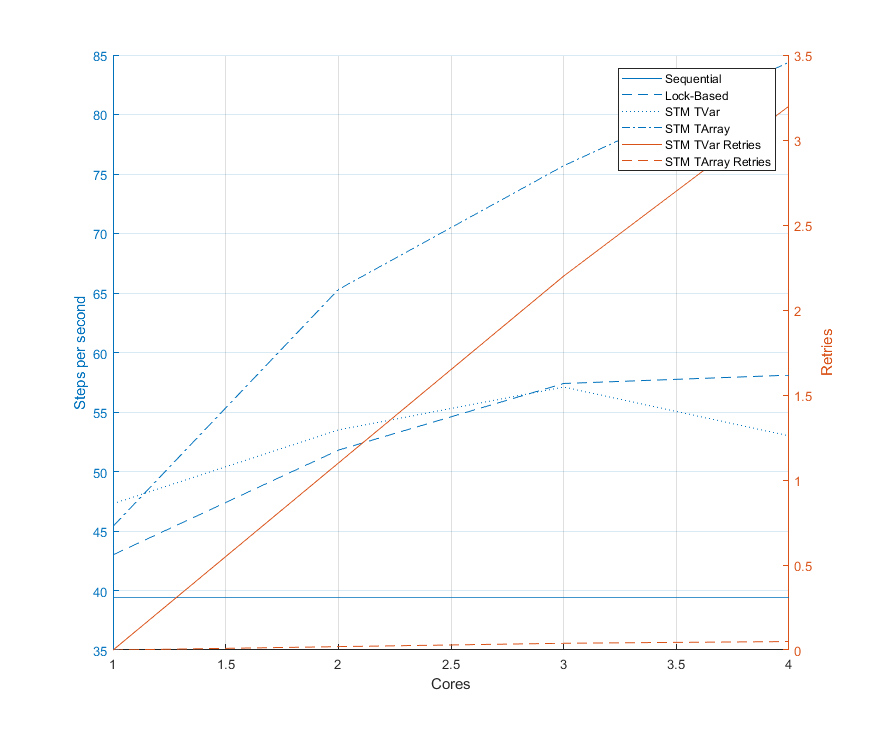
\includegraphics[width=0.7\textwidth, angle=0]{./fig/concurrentabs/sugarscape/varying_cores.png}
	\caption{Steps per second and retries on 50x50 grid and 500 initial agents on varying cores.}
	\label{fig:varying_cores}
\end{figure}

As expected, the \textit{Sequential} implementation is the slowest, followed by the \textit{Lock-Based} and \textit{TVar} approach whereas \textit{TArray} is the best performing one.

We clearly see that using a \textit{TVar} to share the environment is a very inefficient choice in this model: \textit{every} write to a cell leads to a retry independent whether the reading agent reads that changed cell or not, because the data-structure can not distinguish between individual cells. By using a \textit{TArray} we can avoid the situation where a write to a cell in a far distant location of the environment will lead to a retry of an agent which never even touched that cell. Also the \textit{TArray} seems to scale up by 10 steps per second for every core added. It will be interesting to see how far this could go with the Amazon experiment, as we seem not to hit a limit with 4 cores yet.

The inefficiency of \textit{TVar} is also reflected in the nearly similar performance of the \textit{Lock-Based} implementation which even outperforms it on 4 cores. This is due to very similar approaches because both operate on the whole environment instead of only the cells as \textit{TArray} does. This seems to be a bottleneck in \textit{TVar} reaching the best performance on 3 cores, which then drops on 4 cores due to an increasing retries ratio. The \textit{Lock-Based} approach seems to reduce its returns on increased number of cores hitting a limit at 4 cores as well.

\subsection{Scaling up Agents}
So far we kept the initial number of agents at 500, which due to the model specification, quickly drops and stabilises around 200 due to the carrying capacity of the environment as described in the book \cite{epstein_growing_1996} section \textit{Carrying Capacity} (p. 30).

We now want to measure the performance of our approaches under increased number of agents. For this we slightly change the implementation: always when an agent dies it spawns a new one which is inspired by the ageing and birthing feature of Chapter III in the book \cite{epstein_growing_1996}. This ensures that we keep the number of agents roughly constant (still fluctuates but doesn't drop to low levels) over the whole duration. This ensures a constant load of concurrent agents interacting with each other and demonstrates also the ability to terminate and create concurrent agents (threads) dynamically during the simulation.

Except for the \textit{Sequential} approach we ran all experiments with 4 cores (TVar with 3 as well). We looked into the performance of 500, 1,000, 1,500, 2,000 and 2,500 (maximum possible capacity of the 50x50 environment). The results are reported in Table \ref{tab:state_results_agentsscale_time} and plotted in Figure \ref{fig:state_results_agentsscale_time}.

\begin{table}
	\centering
  	\begin{tabular}{ c || c | c | c | c | c }
        Agents  & Sequential & Lock-Based & TVar (3 cores) & TVar (4 cores) & TArray  \\ \hline \hline 
    	    500     & 14.4       & 20.2		  &	20.1           & 18.5       	& \textbf{71.9}    \\ \hline
   		1,000   & 6.8        & 10.8 	      & 10.4           & 9.5         & \textbf{54.8}    \\ \hline
   		1,500   & 4.7        & 8.1 		  & 7.9            & 7.3			& \textbf{44.1}    \\ \hline
   		2,000   & 4.4        & 7.6 		  & 7.4            & 6.7    		& \textbf{37.0}    \\ \hline 
   		2,500   & 5.3        & 5.4 		  & 9.2            & 8.9			& \textbf{33.3}    \\ \hline \hline
   	\end{tabular}
  	
  	\caption{Steps per second on 50x50 grid with varying number of agents with 4 (and 3) cores except Sequential (1 core).}
	\label{tab:state_results_agentsscale_time}
\end{table}

\begin{figure}
	\centering
	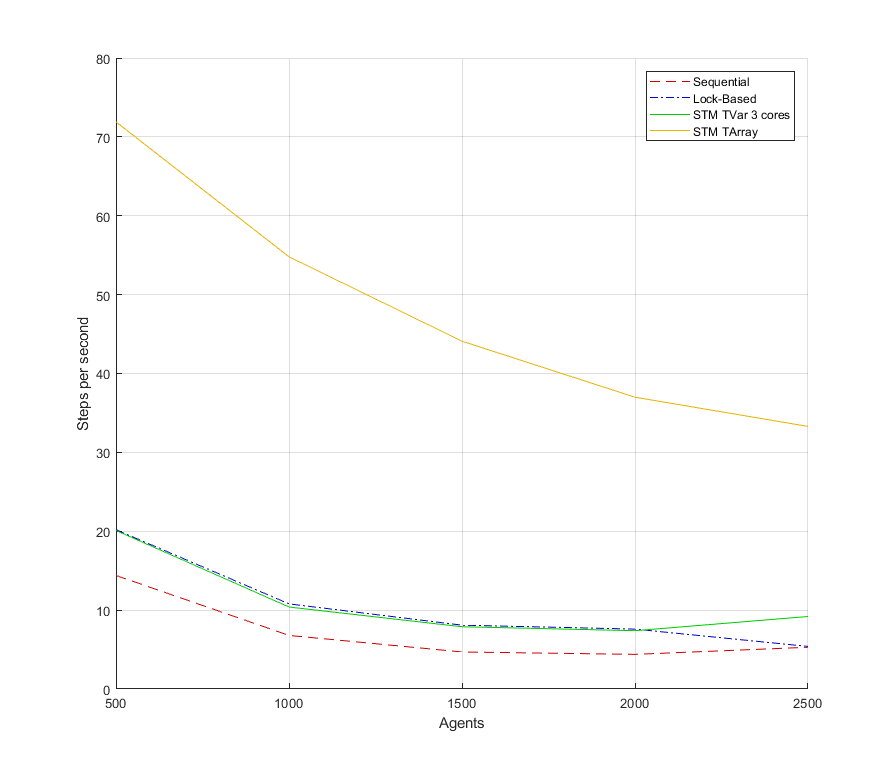
\includegraphics[width=1.0\textwidth, angle=0]{./fig/concurrentabs/sugarscape/varying_agents.png}
	\caption{Steps per second on 50x50 grid and varying number of agents with 4 (and 3) cores except Sequential (1 core).}
	\label{fig:state_results_agentsscale_time}
\end{figure}

As expected, the \textit{TArray} implementation outperforms all others substantially. Also as expected, the \textit{TVar} implementation on 3 cores is faster than on 4 cores as well when scaling up to more agents. The \textit{Lock-Based} approach performs about the same as the \textit{TVar} on 3 cores because of the very similar approaches: both access the \textit{whole} environment. Still the \textit{TVar} approach uses one core less to arrive at the same performance, thus strictly speaking outperforming the \textit{Lock-Based} implementation.

What seems to be very surprising is that in the \textit{Sequential} and \textit{TVar} cases the performance with 2,500 agents is \textit{better} than the one with 2,000 agents. The reason for this is that in the case of 2,500 agents, an agent can't move anywhere because all cells are already occupied. In this case the agent won't rank the cells in order of their pay-off (max sugar) to move to but just stays where it is. We hypothesize that due to Haskells laziness the agents actually never look at the content of the cells in this case but only the number which means that the cells themselves are never evaluated which further increases performance. This leads to the better performance in case of \textit{Sequential} and \textit{TVar} because both exploit laziness.
In the case of the \textit{Lock-Based} approach we still arrive at a lower performance because the limiting factor are the unconditional locks. In the case of the \textit{TArray} approach we also arrive at a lower performance because it seems that STM perform reads on the neighbouring cells which are not subject to lazy evaluation. In Haskell it is notoriously difficult to reason about efficiency (see Chapter \ref{ch:drawbacks} for a short discussion on drawbacks) and this behaviour of improved performance due to Haskells lazyness is no exception. We leave an in-depth investigation for further research as it is beyond the focus of this chapter.

We also measured the average retries both for \textit{TVar} and \textit{TArray} under 2,500 agents where the \textit{TArray} approach shows best scaling performance with 0.01 retries whereas \textit{TVar} averages at 3.28 retries. Again this can be attributed to the better transactional data-structure which reduces retry-ratio substantially to near-zero levels.

\subsection{Going Large-Scale}
To test how far we can scale up the number of cores in both the \textit{Lock-Based} and \textit{TArray} cases, we ran the two experiments (carrying capacity and rebirthing) on Amazon EC2 instances with increasing number of cores starting with 16 and 32 to see if we run into decreasing returns. The results are reported in Table \ref{tab:sug_varying_cores_amazon}.

\begin{table}
	\centering
%  	\begin{tabular}{ c || c | c | c }
%                   & Cores & Carrying Capacity & Rebirthing  \\ \hline \hline 
%    	Lock-Based & 16    & 53.9              & 4.4         \\ \hline
%    	Lock-Based & 32    & 44.2              & 3.6         \\ \hline \hline 
%   		
%   		STM TArray & 16    & \textbf{116.8} (0.23)      & \textbf{39.5} (0.08) \\ \hline
%   		STM TArray & 32    & 109.8 (0.41)      & 31.3 (0.18) \\ \hline \hline 
%   	\end{tabular}
  	
	\begin{tabular}{cc|c|c}
		\multicolumn{1}{ c||  }{\multirow{2}{*}{} } &
		\multicolumn{1}{ |c| }{Cores} & Carrying Capacity    & Rebirthing       \\ \hline \hline 
		
		\multicolumn{1}{ c||  }{\multirow{2}{*}{Lock-Based} } &
		\multicolumn{1}{ |c| }{16} & 53.9              & 4.4       \\ \cline{2-4}
		\multicolumn{1}{ c||  }{}                       &
		\multicolumn{1}{ |c| }{32} & 44.2              & 3.6      \\ \hline \hline 
		
		\multicolumn{1}{ c||  }{\multirow{2}{*}{STM TArray} } &
		\multicolumn{1}{ |c| }{16} & \textbf{116.8} (0.23)      & \textbf{39.5} (0.08)       \\ \cline{2-4}
		\multicolumn{1}{ c||  }{}                       &
		\multicolumn{1}{ |c| }{32} & \textbf{109.8} (0.41)      & \textbf{31.3} (0.18)      \\ \hline \hline 
	\end{tabular}  	
  	
  	\caption{Steps per second on varying cores on Amazon S2 Services.}
	\label{tab:sug_varying_cores_amazon}
\end{table}

As expected, the \textit{Lock-Based} approach doesn't scale up to many cores because each additional core brings more contention to the lock, resulting in even more decreased performance. This is particularly obvious in the rebirthing experiment because of the much larger number of concurrent agents. The \textit{TArray} approach returns better performance on 16 cores but fails to scale further up to 32 where the performance drops below the one with 16 cores. We indicated the retry-ratio in brackets and see that they roughly double from 16 to 32, which is the reason why performance drops as at this point. 

%the INCREASE in time can only happen due to more retries
%Carrying Capacity 16 core ~ 0.23 retry-ratio
%Carrying Capacity 32 core ~ 0.41 retry-ratio
%
%Rebirthing 16 core ~ 0.08 retry-ratio
%Rebirthing 32 core ~ 0.18 retry-ratio

\subsection{Comparison with other approaches}
The paper \cite{lysenko_framework_2008} reports a performance of 17 steps in RePast, 18 steps in MASON (both non-parallel) and 2,000 steps per second on a GPU on a 128x128 grid. Although our \textit{Sequential} implementation, which runs non-parallel as well, outperforms the RePast and MASON implementations of \cite{lysenko_framework_2008}, one must be very well aware that these results were generated in 2008, on current hardware of that time.

%When we run the SugarScape example of RePast with the same model parameters as ours on the same machine (see Table \ref{tab:machine_specs}) we arrive at roughly 450 steps per second - a factor of about 3.8 faster than even our STM \textit{TArray} implementation on 16 cores. This might seem quite shocking, even more so because RePast also performs visual output, rendering the SugarScape in every step. When scaling up the agents to 2,500 the RePast version arrives around roughly 95 steps per second which is still faster by a factor of 3 than our 4 core \textit{TArray} implementation. We attribute this substantial performance difference to the inherent performance difference of functional programming to imperative approaches as already outlined in the previous section. 

The very high performance on the GPU does not concern us here as it follows a very different approach than ours. We focus on speeding up implementations on the CPU as directly as possible without locking overhead. When following a GPU approach one needs to map the model to the GPU which is a delicate and non-trivial matter. With our approach we show that speed up with concurrency is very possible without the low-level locking details or the need to map to GPU. Also some features as bilateral trading between agents, where a pair of agents needs to come to a conclusion over multiple synchronous steps, is difficult to implement on a GPU whereas this is easily possible using STM.

Note that we kept the grid-size constant because we implemented the environment as a single agent which works sequentially on the cells to regrow the sugar. Obviously this doesn't really scale up on parallel hardware and experiments which we haven't included here due to lack of space, show that the performance goes down dramatically when we increase the environment to 128x128 with same number of agents which is the result of Amdahl's law where the environment becomes the limiting factor of the simulation. Depending on the underlying data-structure used for the environment we have two options to solve this problem. In the case of the \textit{Sequential} and \textit{TVar} implementation we build on an indexed array, which we can be updated in parallel using the existing data-parallel support in Haskell. In the case of the \textit{TArray} approach we have no option but to run the update of every cell within its own thread. We leave both for further research as it is out of scope of this paper.

\subsection{Discussion}
This case study showed clearly that besides being substantially faster than the \textit{Sequential} implementation, \textit{STM} is also able to perform considerably better than a \textit{Lock-Based} approach even in the case of a model with much higher complexity in agent behaviour and dramatically increased number of writes to the environment.
Further, this case study demonstrated that the selection of the right transactional data-structure is of fundamental importance when using \textit{STM}. Selecting the right transactional data-structure is very model-specific and can lead to dramatically different performance results.
In this case the \textit{TArray} performed best due to many writes but in the SIR case-study a \textit{TVar} showed good enough results due to the very low number of writes. When not carefully selecting the right transactional data-structure which supports fine-grained concurrency, a lock-based implementation might perform as well or even outperform the STM approach as can be seen when using the \textit{TVar}.
Although the \textit{TArray} is the better transactional data-structure overall, it might come with an overhead, performing worse on low number of cores than a \textit{TVar} approach but has the benefit of quickly scaling up to multiple cores. Depending on the transactional data-structure, scaling up to multiple cores hits a limit at some point. In the case of the \textit{TVar} the best performance is reached with 3 cores. With the \textit{TArray} we reached this limit around 16 cores.

Note that the comparison between the \textit{Lock-Based} approach and the \textit{STM TArray} implementation is a bit unfair due to a very different locking structure. A more suitable comparison would have been to use an indexed Array with a tuple of (MVar, IORef) in each cell to support fine-grained locking on cell-level. This would be a more just comparison to the \textit{STM Array} where fine-grained transactions happen on the cell-level. We hypothesize that \textit{STM} will still outperform the \textit{IO} approach but to a lesser degree - we leave the proof of this for further research.

%Unfortunately, for this model the performance is nowhere comparable to imperative approaches, which we attribute to the inherent performance difference of functional programming to imperative approaches. With the use of advanced language features we might arrive at much improved performance but we leave this for further research as we focus primarily on the comparison between lock-based and STM approaches.

%we can implement everything except synchronous direct agent-interactions atm: if agent-interaction is one-way e.g. paying back a loan then this is no problem. thus the following parts of the Sugarscape are not possible with our current STM approach: mating, trading and lending  because all 3 require direct agent-to-agent interaction over multiple steps. We leave the problem of developing such an algorithm / implementation for further research.

\section{Parallel Runs}
Often one needs to perform a large number of runs of the same simulation. The most prominent use-cases for this are:

\begin{itemize}
	\item Parameter Sweeps / Variations - to explore the parameter space and the dynamics under varying parameter configurations, the same simulation is run with varying parameters and the results recorded for statistical analysis.
	
	\item Stochastic replications - due to ABS stochastic nature, running a simulation only once does not allow to generalise or predict overall behaviour - one might have just hit an (un)fortunate special case. To counter this problem, in ABS multiple replications of the  simulation are run with same initial model parameters but with different random-number streams. All the results are collected and analysed stochastically (averaged, median,...) from which then more general properties can be derived.
\end{itemize}

In each case thousands of runs of the same simulation with different model parameters and / or varying random-number streams are needed, requiring a considerable amount of computing power.

Parallelism is a remedy to this problem because in each of these cases individual runs do not interfere with each other and thus can be seen as isolated from each other, like referential transparent, pure computations. Our approaches shown in Part II make this very explicit: the top level functions can always be made pure computations because we are ruling out \textit{IO} and thus even though Monads are employed in many cases, they are still pure. A benefit of our approach is that it is guaranteed at compile time, that individual runs do not interfere with each other and thus there is no danger that parallel runs influence each other. 

All this allows to implement parameter sweeps and stochastic replications both through evaluation and data-flow parallelism making another very compelling use-case - probably the most striking one - for the use of parallelism in ABS. We hypothesize that data-flow parallelism is better suited for this task because it makes parallelism more explicit as it is indeed a data-flow problem: we pass parameters to single replications which are run and return their results. To apply this we simply run the top level replication logic in the \textit{Par} Monad where replications are run in parallel by forking tasks and results are handed back through \textit{IVars}. If we want the convenience of having a monadic random-number generator within the \textit{Par} Monad, one can use the combined \textit{ParRand} Monad which provides both.

\subsection{Reflection}
Despite high hopes, there were very few opportunities to apply parallelism to our pure functional ABS. This has three reasons: it is often highly model specific and our models simply didn't offer a lot of suitable parallelisations, the data-structures have to support parallelism e.g. map doesn't, but we also have to say that the sequential nature of ABS in general seems to be less suited to parallelism. We will see that concurrency offers a remedy against that.

the difficulties / low ausbeute von parallelism just Shows how difficult it is to parallelise abs. also maybe our approach is not very well.suited e.g. not very functional?

In general we aimed at running agents in parallel using the various techniques. Because of the quite sequential nature of the agent behaviours themselves, there is much less potential for parallelism \textit{within} an agent, thus the obvious idea was to run them all in parallel because they are an obvious unit of partitioning, have considerable workload and can indeed be run in parallel under given circumstances.
Unfortunately it is not possible applying parallelism in case the agents run within a monadic context: we have side-effects which imposes ordering e.g. in the case of a

It becomes apparent, that applying parallelism to our approaches doesn't lead to very much performance increase. This is because in the cases were we can actually run the agents with evaluation parallelism, the performance is not bound by them. As soon as we switch to monadic agents, evaluation parallelism is out of the window, as agents can't be run in parallel anymore because side-effects require to impose a sequential ordering. This can be only tackled using non-deterministic concurrency, which we will show in-depth in the next chapter because it is much more promising than prallelism in terms of performance gain. Further it is also more technically involved and the way we chose to approach it using Software Transactional Memory (STM) hasn't been undertaken in this form ever and to our best knowledge we are the first one to do so.

We see a direct consequence of this that types also reflect the semantics of our model: when our agents are pure they can be run indeed in parallel and independent from each other, if they are monadic, then this is not applicable to parallelism. In the next section, we show how to approach this problem and come up with a solution where we can run monadic agents in parallel. This is obviously only possible within a concurrent setting which means we have to sacrifice determinism in our solution. Still we reach considerable speed ups using Software Transactional Memory.

We didn't discuss data parallelism on large array structure or parallelism on GPU as they are used in massively large numerical computation. These techniques achieve tremendous speed ups but are not applicable to ABS in general but only in model specific cases where e.g. each agent needs to crunch through arrays of numbers to perform numerical computations. We refer to \cite{marlow_parallel_2013} for a more in-depth discussion of both in Haskell and leave the application to pure functional ABS for further research.

\chapter{Concurrent ABS}
\label{ch:concurrent_abs}

%- no comparison to io or repast: the story is "concurrency with compile time guarantees", only mention that an io based single lock performs much worse in sir and slightly worse in sugarscape. leave Array i IORef for further research

In an ideal world, we would like to solve all our problems using parallelism but unfortunately, it can't be applied to all parallel problems and ABS is no exception. As soon as there are data-dependencies, like we have them in the Sugarscape model in the form of the read/write environment and synchronous agent-interactions, and to a lesser extent in the monadic SIR with the \textit{Rand} Monad, we cannot avoid concurrency. More general, this is due to the fact that agents are executed within a monadic context, from which the  sequencing of effectful computations immediately follows - this is the very meaning of the Monad abstraction. Indeed, we have shown both by argument and measurement in the previous chapter the very fact that parallelism is simply not applicable to monadic execution of agents due to sequencing of effects, which renders all attempts of running monadic agents in parallel void. In this chapter we discuss the use of concurrency to run agents which have a monadic context in parallel - which is the only way we can execute monadic agents at the same time.

\medskip

Traditional approaches to concurrency follow a lock-based approach, where sections which access shared data are synchronised through synchronisation primitives like mutexes, semaphores, monitors,... The lock-based path is a well trodden one, with all problems and benefits well established. In this chapter we follow a different path and look into using Software Transactional Memory (STM) for implementing concurrent ABS, which promises to overcome the problems of lock-based approaches. Although STM exists in other languages as well, Haskell was one of the first to natively build it into its core, thus it is a natural choice to follow that direction when already investigating pure functional ABS.

Unfortunately, as soon as we employ concurrency, we lose all static guarantees about reproducibility and the use of STM is no exception. Still, STM has the unique benefit that it can guarantee the lack of persistent side-effects at compile time, allowing unproblematic retries of transactions, something of fundamental importance in STM as will be described below. This implies also another \textit{very} compelling advantage of STM over unrestricted lock-based approaches: by using STM, we can reduce the side-effects allowed substantially and guarantee at compile time, that the differences between runs of same initial conditions will only stem from the fact that we run the simulation concurrently - \textit{and from nothing else}. All this makes the use of STM very compelling and to our best knowledge we are the very first to investigate the use of STM for implementing concurrent ABS in a systematic way.

\medskip

The paper \cite{discolo_lock_2006} gives a good indication how difficult and complex constructing a correct concurrent program is and shows how much easier, concise and less error-prone an STM implementation is over traditional locking with mutexes and semaphores. More important, it shows that STM consistently outperforms the lock-based implementations. We follow this work and compare the performance of lock-based and STM implementations and hypothesise that the reduced complexity and increased performance will be directly applicable to ABS as well.

We present two case studies using the already introduced SIR (Chapter \ref{sec:sir_model}) and Sugarscape (Chapter \ref{sec:sugarscape}) models. We compare the performance of lock-based and STM implementations in each case where we investigate both the scaling performance under increasing number of CPUs and agents. We show that the STM implementations consistently outperform the lock-based ones and scale much better to increasing number of CPUs both on local machines and on Amazon Cloud Services.

%Note that there exists also the actor model of concurrency, which is especially well suited to implement concurrent applications in functional languages. We give a short overview over it, existing research and its use in ABS in the section \ref{sec:actors} but leave it for further research as it has very different implications, which are beyond the focus of this thesis.

\section{Software Transactional Memory}
Software Transactional Memory was introduced by \cite{shavit_software_1995} in 1995 as an alternative to lock-based synchronisation in concurrent programming which, in general, is notoriously difficult to get right. This is because reasoning about the interactions of multiple concurrently running threads and low level operational details of synchronisation primitives is \textit{very hard}. The main problems are \cite{marlow_parallel_2013}:

\begin{itemize}
	\item Race conditions due to forgotten locks;
	\item Deadlocks resulting from inconsistent lock ordering;
	\item Corruption caused by uncaught exceptions;
	\item Lost wake-ups induced by omitted notifications.
\end{itemize}

What is worse, concurrency does not compose. It is very difficult to write two functions (or methods in an object) acting on concurrent data which can be composed into a larger concurrent behaviour. The reason for the difficulty is that one has to know about the internal details of locking, which breaks encapsulation and makes composition dependent on knowledge about their implementation. Therefore, it is impossible to compose two functions where, for example, one withdraws some amount of money from an account and the other deposits this amount of money into a different account. The problem is that one ends up with a temporary state where the money is in neither of the accounts, creating an inconsistency and a potential source for errors because threads can be rescheduled at any time.

STM promises to solve all of these problems for a low cost by executing actions \textit{atomically}, where modifications made in such an action are invisible to other threads and changes by other threads are also invisible until actions are committed - STM actions are atomic and isolated. When an STM action exits, either one of two outcomes happen: if no other thread has modified the same data as the thread running the STM action, then the modifications performed by the action will be committed and become visible to the other threads. If other threads have modified the data then the modifications will be discarded, the action rolled back and automatically restarted.

\subsection{Software Transactional Memory in Haskell}
The work of \cite{harris_composable_2005, harris_transactional_2006} added STM to Haskell, which was one of the first programming languages to incorporate STM with composable operations into its main core. In the Haskell implementation, STM actions run within the \texttt{STM} Monad. This restricts the operations to only STM primitives as shown below. This means that \texttt{STM} actions are always repeatable without persistent side effects because such persistent side effects (for example writing to a file, launching a missile) are not possible in the \texttt{STM} Monad. This is also the fundamental difference to \texttt{IO}, where all bets are off and \textit{everything} is possible because \texttt{IO} can run everything without restrictions.

Thus, the ability to \textit{restart} an action without any persistent effects is only possible due to the nature of Haskell's type system and by restricting the effects to \texttt{STM} only, ensures that only controlled effects, which can be rolled back, occur.

STM comes with a number of primitives to share transactional data. Amongst others the most important ones are:

\begin{itemize}
	\item \texttt{TVar} - a transactional variable which can be read and written arbitrarily;
	
	\item \texttt{TMVar} - a transactional \textit{synchronising} variable which is either empty or full. To read from an empty or write to a full \texttt{TMVar} will cause the current thread to block and retry its transaction when \textit{any} transactional primitive of this action has changed.
	
	\item \texttt{TArray} - a transactional array where each cell is an individual transactional variable \texttt{TVar}, allowing more finer-grained transactions instead of having the whole array in a \texttt{TVar}.
	
	\item \texttt{TChan} - a transactional channel, representing an unbounded FIFO channel, based on a linked list of \texttt{TVar}.
\end{itemize}

Furthermore STM also provides combinators to deal with blocking and composition:

\begin{itemize}
	\item \texttt{retry :: STM ()} retries an \texttt{STM} action. This will cause to abort the current transaction and block the thread it is running in. When \textit{any} of the transactional data primitives have changed, the action will be run again. This is useful to await the arrival of data in a \texttt{TVar}, or put more general, to block on arbitrary conditions. 
	
	\item \texttt{orElse :: STM a $\rightarrow$ STM a $\rightarrow$ STM a} allows us to combine two blocking actions where either one is executed, but not both. The first action is run and if it is successful its result is returned. If it retries, then the second is run and if that one is successful its result is returned. If the second one retries, the whole \texttt{orElse} retries. This can be used to implement alternatives in blocking conditions, which can obviously be nested arbitrarily.
\end{itemize}

To run an \texttt{STM} action the function \texttt{atomically :: STM a $\rightarrow$ IO a} is provided, which performs a series of \texttt{STM} actions atomically within the \texttt{IO} Monad. It takes the \texttt{STM} action, which returns a value of type \texttt{a} and returns an \texttt{IO} action which returns a value of type \texttt{a}. The \texttt{IO} action then can only be executed from within the \texttt{IO} Monad, either within the main thread or an explicitly forked thread.

STM in Haskell is implemented using optimistic synchronisation, which means that instead of locking access to shared data, each thread keeps a transaction log for each read and write to shared data that it makes. When the transaction exits, the thread checks whether it has a consistent view to the shared data or not. It checks whether other threads have written to memory it has read, thus it can identify whether a rollback is required or not.

However, STM does not come without issues. The authors of \cite{perfumo_limits_2008} analyse several Haskell STM programs with respect to their transactional behaviour. They identified the roll-back rate as one of the key metrics, which determines the scalability of an application. Although STM might promise better performance, they also warn of the overhead it introduces, which could be quite substantial in particular for programs which do not perform much work inside transactions as their commit overhead is high.

\subsection{STM Examples}
We provide two examples to demonstrate the use and semantics of STM. The first example is an implementation of the aforementioned functionality, where money is withdrawn from one account and transferred to another. The implementing function \texttt{transferFunds} takes two \texttt{TVar}, holding the account balances, and the amount to exchange. It executes using \texttt{atomically}, therefore running in the \texttt{IO} Monad. It uses the two functions \texttt{withdraw} and \texttt{deposit} which do the work of withdrawing some amount from one account and depositing some amount to another. This example demonstrates how easily STM can be used: the implementation looks quite straightforward, simply swapping values, without any locking involved or special handling of concurrency, other than the use of \texttt{atomically}.

\begin{HaskellCode}
transferFunds :: TVar Integer -> TVar Integer -> Integer -> IO ()
transferFunds from to n = atomically (do
  withdraw from n
  deposit to n)
  
withdraw :: TVar Integer -> Integer -> STM ()
withdraw account amount = do
  balance <- readTVar account
  writeTVar (balance - amount)
  
deposit :: TVar Integer -> Integer -> STM ()
deposit account amount = do
  balance <- readTVar account
  writeTVar (balance + amount)
\end{HaskellCode}

In the second example we show the retry semantics of STM, by using it within a \texttt{StateT} transformer where \texttt{STM} is the innermost Monad. It is important to understand that \texttt{STM} does not provide a transformer instance for very good reasons. If it would provide a transformer then we could make \texttt{IO} the innermost Monad and perform \texttt{IO} actions within \texttt{STM}. This would violate the retry semantics, as in case of a retry, \texttt{STM} is unable to undo the effects of \texttt{IO} actions in general. This stems from the fact that the \texttt{IO} type is simply too powerful and we cannot distinguish between different kinds of \texttt{IO} actions in the type, be it simply reading from a file or actually launching a missile. Let's look at the example code:

\begin{HaskellCode}
stmAction :: TVar Int -> StateT Int STM Int 
stmAction v = do
  -- print a debug output and increment the value in StateT 
  Debug.trace "increment!" (modify (+1))
  -- read from the TVar
  n <- lift (readTVar v)
  -- await a condition: content of the TVar >= 42
  if n < 42
    -- condition not met: retry
    then lift retry
    -- condition met: return content ot TVar
    else return n
\end{HaskellCode}

In this example, the \texttt{STM} is the innermost Monad in a stack with a \texttt{StateT} transformer. When \texttt{stmAction} is run, it prints an \texttt{'increment!'} debug message to the console and increments the value in the \texttt{StateT} transformer. Then it awaits a condition. For as long as \texttt{TVar} is less then 42 the action will retry whenever it is run. If the condition is met, it will return the content of the \texttt{TVar}. We see the combined effects of using the transformer stack where we have both the \texttt{StateT} and the \texttt{STM} effects available. The question is how this code behaves if we actually run it. To do this we need to spawn a thread:

\begin{HaskellCode}
stmThread :: TVar Int -> IO ()
stmThread v = do
  -- the initial state of the StateT transformer
  let s = 0
  -- run the state transformer with initial value of s (0)
  let ret = runStateT (stmAction v) s
  -- atomically run the STM block
  (a, s') <- atomically ret
  -- print final result
  putStrLn("final StateT state     = " ++ show s' ++
           ", STM computation result = " ++ show a)
\end{HaskellCode}

The thread simply runs the \texttt{StateT} transformer layer with the initial value of 0 and then the \texttt{STM} computation through \texttt{atomically} and prints the result to the console. The value of \texttt{a} is the result of \texttt{stmAction} and \texttt{s'} is the final state of the \texttt{StateT} computation. To actually run this example we need the main thread to update the \texttt{TVar} until the condition is met within \texttt{stmAction}:

\begin{HaskellCode}
main :: IO ()
main = do
  -- create a new TVar with initial value of 0
  v <- newTVarIO 0 
  -- start the stmThread and pass the TVar
  forkIO (stmThread v)
  -- do 42 times...
  forM_ [1..42] (\i -> do
    -- use delay to 'make sure' that a retry is happening for ever increment
    threadDelay 10000
    -- write new value to TVar using atomically
    atomically (writeTVar v i))
\end{HaskellCode}

If we run this program, we will see \texttt{'increment!'} printed 43 times, followed by \texttt{'final StateT state = 1, STM computation result = 42'}. This clearly demonstrates the retry semantics where \texttt{stmAction} is retried 42 times and thus prints \texttt{'increment!'} 43 times to the console. The \texttt{StateT} computation, however, is carried out only once and is always rolled back when a retry is happening. The rollback is easily possible in pure functional programming due to persistent data structure, by simply throwing away the new value and retrying with the original value. This example also demonstrates that any \texttt{IO} actions which happen within an \texttt{STM} action are persistent and can obviously not be rolled back. \texttt{Debug.trace} is an \texttt{IO} action masked as pure using \texttt{unsafePerformIO}.

\section{Software Transactional Memory in ABS}
\label{sec:stm_abs}
In this section we give a short overview of how we apply STM to pure functional ABS. In both case studies we fundamentally follow a time-driven, parallel approach as introduced in Chapter \ref{sub:par_strategy}, where the simulation is advanced by a given $\Delta t$ and in each step all agents are executed. To employ parallelism, each agent runs within its own thread and agents are executed in lock-step, synchronising between each $\Delta t$, which is controlled by the main thread. See Figure \ref{fig:stm_abs_structure} for a visualisation of the concurrent, parallel time-driven lock-step approach.

By running each agent in a thread will guarantee the execution in parallel even if the agent has a monadic context. This forces us to evaluate each agents monadic context separately instead of running them all in a common context. This means that we are ending up in the \texttt{IO} Monad because \texttt{STM} can be only transacted from within an \texttt{IO} context due to non-deterministic side effects. This is no contradiction to our original claim. Yes we are running in \texttt{IO} but not the agent behaviour itself, which is a fundamental difference.

An agent thread will block until the main thread sends the next $\Delta t$ and runs the \texttt{STM} action atomically with the given $\Delta t$. When the \texttt{STM} action has been committed, the thread will send the output of the agent action to the main thread to signal it has finished. The main thread awaits the results of all agents to collect them for output of the current step, for example visualisation or writing to a file.

As will be described in subsequent sections, central to both case studies is an environment which is shared between the agents using a \texttt{TVar} or \texttt{TArray} primitive, through which the agents communicate concurrently with each other. To get the environment in each step for visualisation purposes, the main thread can access the \texttt{TVar} and \texttt{TArray} as well. 

\begin{figure}
	\centering
	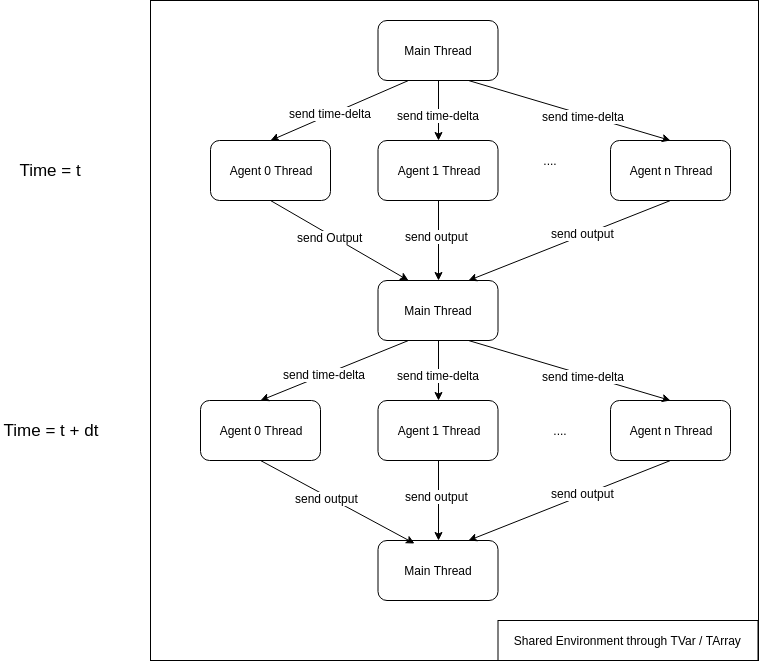
\includegraphics[width=0.7\textwidth, angle=0]{./fig/concurrentabs/stm_abs.png}
	\caption[Diagram of the parallel time-driven lock-step approach]{Diagram of the parallel time-driven lock-step approach.}
	\label{fig:stm_abs_structure}
\end{figure}

\subsection{Adding STM to agents}
We briefly discuss how to add STM to agents on a technical level and also show how to run them within their own threads. We use the SIR implementation as example - applying it to the Sugarscape implementation works exactly the same way and is left as a trivial exercise to the reader.

The first step is to simply add the \texttt{STM} Monad as the innermost level to the already the existing Transformer stack. Further, the environment is now passed as a transactional data primitive to the agent at \textit{construction time}. Thus, the agent does not receive the \texttt{SIREnv} as input any more but receives it through currying when constructing its initial \texttt{MSF}. Further, the agent modifies the \texttt{SIREnv} directly through the \texttt{TVar}, as demonstrated in the case of the infected agent.

\begin{HaskellCode}
-- Make Rand a transformer to be able to add STM as innermost monad
type SIRMonad g = RandT g STM
-- Input to agent is now an empty tuple instead of the Environment
type SIRAgent g = SF (SIRMonad g) () SIRState

-- The MSF construction function takes now the TVar with the environment.
sirAgent :: RandomGen g => TVar SIREnv -> Disc2dCoord -> SIRState -> SIRAgent g

-- The infected agent behaviour is nearly the same except that
-- the agent modifies the environment through the TVar
infected :: RandomGen g => SF (SIRMonad g) () (SIRState, Event ())
infected = proc _ -> do
  recovered <- occasionally illnessDuration () -< ()
  if isEvent recovered
    then (do
      -- update the environment through the TVar
      arrM_ (lift $ lift $ modifyTVar env (changeCell coord Recovered)) -< ()
      returnA -< (Recovered, Event ()))
    else returnA -< (Infected, NoEvent)
\end{HaskellCode}

The agent thread is straightforward. It takes \texttt{MVar} synchronisation primitives to synchronise with the main thread and simply runs the agent behaviour each time it receives the next \textit{DTime}:

\begin{HaskellCode}
agentThread :: RandomGen g 
            => Int             -- ^ Number of steps to compute
            -> SIRAgent g      -- ^ Agent behaviour MSF
            -> g               -- ^ Random-number generator of the agent
            -> MVar SIRState   -- ^ Synchronisation back to main thread
            -> MVar DTime      -- ^ Receiving DTime for next step
            -> IO ()
agentThread 0 _ _ _ _ = return () -- all steps computed, terminate thread
agentThread n sf rng retVar dtVar = do
  -- wait for dt to compute current step
  dt <- takeMVar dtVar

  -- compute output of current step
  let sfReader = unMSF sf ()
      sfRand   = runReaderT sfReader dt
      sfSTM    = runRandT sfRand rng
  -- run the STM action atomically within IO
  ((ret, sf'), rng') <- atomically sfSTM 

  -- post result to main thread
  putMVar retVar ret
  
  -- tail recursion to next step 
  agentThread (n - 1) sf' rng' retVar dtVar
\end{HaskellCode}

Computing a simulation step is now trivial within the main thread. All agent threads \texttt{MVars} are signalled to unblock followed by an immediate block on the \texttt{MVars} into which the agent threads post back their result. The state of the current step is then extracted from the environment, which is stored within the \texttt{TVar} which the agent threads have updated.

\begin{HaskellCode}
simulationStep :: TVar SIREnv     -- ^ environment 
               -> [MVar DTime]    -- ^ sync dt to threads
               -> [MVar SIRState] -- ^ sync output from threads
               -> DTime           -- ^ time delta
               -> IO SIREnv
simulationStep env dtVars retVars dt = do
  -- tell all threads to continue with the corresponding DTime
  mapM_ (`putMVar` dt) dtVars
  -- wait for results but ignore them, SIREnv contains all states
  mapM_ takeMVar retVars
  -- return state of environment when step has finished
  readTVarIO env
\end{HaskellCode}

The difference to an implementation which uses \texttt{IO} are minor but far reaching. Instead of using \texttt{STM} as innermost Monad, we use \texttt{IO}, thus running the whole agent behaviour within the \texttt{IO} Monad. Instead of receiving the environment through a \texttt{TVar}, the agent receives it through an \texttt{IORef}. It also receives an \texttt{MVar} which is the synchronisation primitive to synchronise the access to the environment in the \texttt{IORef} amongst all agents. Agents grab and release the synchronisation lock of the \texttt{MVar} when they enter and leave a critical section in which they operate on the environment stored in the \texttt{IORef}.

\section{Case Study I: SIR}
\label{sec:concurrent_sir}
Our first case study is the SIR model as introduced in Chapter \ref{sec:sir_model}. The aim of this case study is to investigate the potential speed up a concurrent \textit{STM} implementation gains over a sequential one under varying number of CPU cores and agents. The behaviour of the agents is quite simple and the interactions are happening indirectly through the environment, where reads from the environment outnumber the writes to it by far. Further, a comparison to a lock-based implementation with the \textit{IO} Monad is done to understand that \textit{STM} is also able to outperform traditional concurrency, \textit{in a pure functional ABS setting} while still retaining its greater static guarantees than \textit{IO} \footnote{The code of all three implementations is available at \url{https://github.com/thalerjonathan/phd/tree/master/public/stmabs/code/SIR}}.

\begin{enumerate}
	\item Sequential - this is the original implementation as discussed in Chapter \ref{sec:adding_env}, where the discrete 2D environment is shared amongst all agents as read-only data and the agents are executed sequentially within the main thread without any concurrency.
	\item STM - this is the same implementation as the \textit{Sequential} one but agents run now in the \textit{STM} Monad and have access to the discrete 2D environment through a transactional variable \textit{TVar}. This means that the agents now communicate indirectly by reads and writes through the \textit{TVar}.
	\item Lock-Based - this follows the \textit{STM} implementation, with the agents running in \textit{IO}. They share the discrete 2D environment using an \textit{IORef} and have access to an \textit{MVar} lock to synchronise access to it.
\end{enumerate}

Each experiment was run until $t = 100$ and stepped using $\Delta t = 0.1$. For each experiment we conducted 8 runs on our machine (see Table \ref{tab:machine_specs}) under no additional work-load and report the mean. %Further, we checked the visual outputs and the dynamics and they look qualitatively the same as the reference \textit{Sequential}. We could have used more rigour and properly validated the implementations against the formal specification using tests as we do in Chapter Property-based testing but we leave this for further res.
In the experiments we varied the number of agents (grid size) as well as the number of cores when running concurrently - the numbers are always indicated clearly.

\begin{table}
	\centering
	\begin{tabular}{ c || c }
		OS & Fedora 28, 64-bit \\ \hline
		RAM & 16 GByte \\ \hline
		CPU & Intel i5-4670K @ 3.4GHz \\ \hline
		HD & 250Gbyte SSD \\ \hline
		Haskell & GHC 8.2.2
	\end{tabular}
	
	\caption{Machine and Software specs for all experiments}
	\label{tab:machine_specs}
\end{table}

\subsection{Constant Grid Size, Varying Cores}
In this experiment we held the grid size constant to 51 x 51 (2,601 agents) and varied the cores. The results are reported in Table \ref{tab:constgrid_varyingcores}.

\begin{table}
	\centering
	\begin{tabular}{cc|c}
		\multicolumn{1}{ c||  }{\multirow{2}{*}{} } &
		\multicolumn{1}{ |c| }{Cores} & Duration      \\ \hline \hline 
		
		\multicolumn{1}{ c||  }{\multirow{1}{*}{Sequential} } &
		\multicolumn{1}{ |c| }{1} & 72.5      \\ \hline \hline 
		
		\multicolumn{1}{ c||  }{\multirow{4}{*}{Lock-Based} } &
		\multicolumn{1}{ |c| }{1} & 60.6       \\ \cline{2-3}
		\multicolumn{1}{ c||  }{}                       &
		\multicolumn{1}{ |c| }{2} & 42.8    \\ \cline{2-3}
		\multicolumn{1}{ c||  }{}                       &
		\multicolumn{1}{ |c| }{3} & 38.6    \\ \cline{2-3}
		\multicolumn{1}{ c||  }{}                       &
		\multicolumn{1}{ |c| }{4} & 41.6    \\ \hline \hline 
		
		\multicolumn{1}{ c||  }{\multirow{4}{*}{STM} } &
		\multicolumn{1}{ |c| }{1} & 53.2       \\ \cline{2-3}
		\multicolumn{1}{ c||  }{}                       &
		\multicolumn{1}{ |c| }{2} & 27.8    \\ \cline{2-3}
		\multicolumn{1}{ c||  }{}                       &
		\multicolumn{1}{ |c| }{3} & 21.8    \\ \cline{2-3}
		\multicolumn{1}{ c||  }{}                       &
		\multicolumn{1}{ |c| }{4} & \textbf{20.8}    \\ \hline \hline 
	\end{tabular}
  	
  	\caption{Experiments on 51x51 (2,601 agents) grid with varying number of cores. Timings in seconds (lower is better).}
	\label{tab:constgrid_varyingcores}
\end{table}

The \textit{STM} implementation running on 4 cores shows a speed up factor of 3.6 over \textit{Sequential}, which is a quite impressive number when considering that we can achieve at most a factor of 4 when running on 4 cores. It seems that \textit{STM} allow us to push the practical limit very close to the theoretical one, whereas the \textit{Lock-Based} approach just arrives at a factor of 1.74 on 4 cores.

Comparing the performance and scaling to multiple cores shows that the \textit{STM} implementation significantly outperforms the \textit{Lock-Based} one and scales better to multiple cores. The \textit{Lock-Based} implementation performs best with 3 cores and shows slightly worse performance on 4 cores as can be seen in Figure \ref{fig:core_duration_stm_io}. This is no surprise because the more cores are running at the same time, the more contention for the lock, thus the more likely synchronisation happening, resulting in higher potential for reduced performance. This is not an issue in \textit{STM} because no locks are taken in advance. 

\begin{figure}
	\centering
	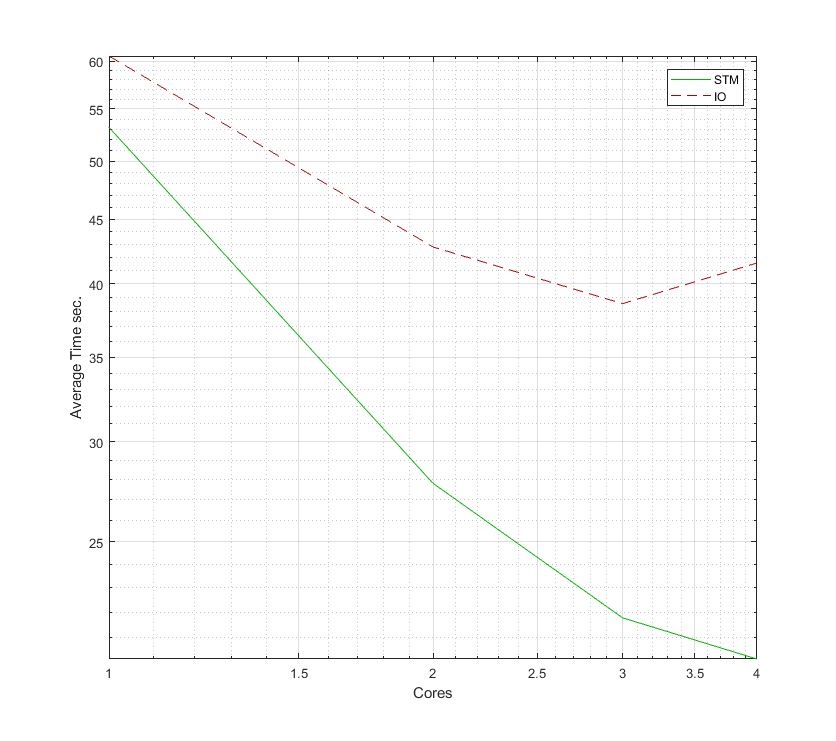
\includegraphics[width=0.8\textwidth, angle=0]{./fig/concurrentabs/sir/core_duration_stm_io.png}
	\caption{Comparison of performance and scaling on multiple cores of STM and Lock-Based. Note that the Lock-Based implementation seems to perform slightly worse on 4 than on 3 cores probably due to lock-contention.}
	\label{fig:core_duration_stm_io}
\end{figure}

\subsection{Varying Grid Size, Constant Cores}
In this experiment we varied the grid size and used always 4 cores. The results are reported in Table \ref{tab:varyinggrid_constcores} and plotted in Figure \ref{fig:varyinggrid_constcores}.

\begin{table}
	\centering
  	\begin{tabular}{ c || c | c | c }
        Grid-Size          & STM              & Lock-Based   & Ratio \\ \hline \hline 
   		51 x 51 (2,601)    & \textbf{20.2}    & 41.9         & 2.1 \\ \hline
   		101 x 101 (10,201) & \textbf{74.5}    & 170.5        & 2.3 \\ \hline
   		151 x 151 (22,801) & \textbf{168.5}   & 376.9        & 2.2 \\ \hline
   		201 x 201 (40,401) & \textbf{302.4}   & 672.0        & 2.2 \\ \hline
   		251 x 251 (63,001) & \textbf{495.7}   & 1,027.3      & 2.1 \\ \hline \hline
  	\end{tabular}

  	\caption{Performance on varying grid sizes. Timings in seconds (lower is better). Ratio compares STM to Lock-Based.}
	\label{tab:varyinggrid_constcores}
\end{table}

It is clear that the \textit{STM} implementation outperforms the \textit{Lock-Based} implementation by a substantial factor.

\begin{figure}
	\centering
	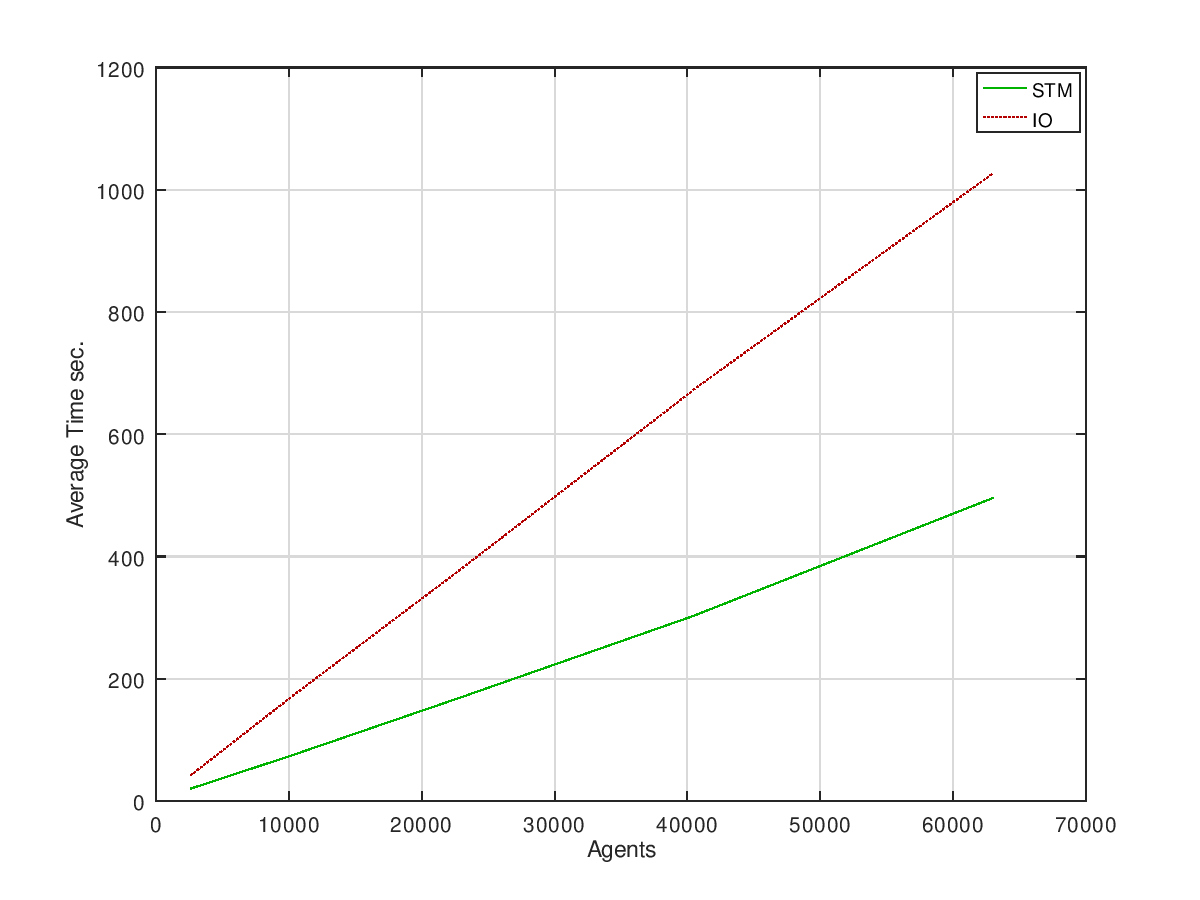
\includegraphics[width=1\textwidth, angle=0]{./fig/concurrentabs/sir/stm_io_varyinggrid_performance.png}
	\caption{Performance on varying grid sizes.}
	\label{fig:varyinggrid_constcores}
\end{figure}

\subsection{Retries}
Of very much interest when using STM is the retry-ratio, which obviously depends highly on the read-write patterns of the respective model. We used the \textit{stm-stats} library to record statistics of commits, retries and the ratio. The results are reported in Table \ref{tab:retries_stm}.

\begin{table}
	\centering
  	\begin{tabular}{ c || c | c | c }
        Grid-Size 		   & Commits    & Retries & Ratio \\ \hline \hline 
   		51 x 51 (2,601)    & 2,601,000  & 1306.5  & 0.0 \\ \hline
   		101 x 101 (10,201) & 10,201,000 & 3712.5  & 0.0 \\ \hline
   		151 x 151 (22,801) & 22,801,000 & 8189.5  & 0.0 \\ \hline
   		201 x 201 (40,401) & 40,401,000 & 13285.0 & 0.0 \\ \hline 
   		251 x 251 (63,001) & 63,001,000 & 21217.0 & 0.0 \\ \hline \hline
  	\end{tabular}
  	
  	\caption{Retry ratios on varying grid sizes on 4 cores.}
	\label{tab:retries_stm}
\end{table}

Independent of the number of agents we always have a retry-ratio of 0.0. This indicates that this model is \textit{very} well suited to STM, which is also directly reflected in the much better performance over the \textit{Lock-Based} implementation. Obviously this ratio stems from the fact that in our implementation we have \textit{very} few writes, which happen only in case when an agent changes from Susceptible to Infected or from Infected to Recovered. On the other hand, there are a very large number of reads due to indirect agent interaction. For \textit{STM} this is no problem because no lock is taken but the \textit{Lock-Based} approach is forced to conservatively take the lock to ensure mutual exclusive access to the critical section across all agents.

\subsection{Going Large-Scale}
To test how far we can scale up the number of cores in both the \textit{Lock-Based} and \textit{STM} cases, we ran two experiments, 51x51 and 251x251, on Amazon EC2 instances with a larger number of cores than our local machinery, starting with 16 and 32 to see if we are running into decreasing returns. The results are reported in Table \ref{tab:sir_varying_cores_amazon}.

\begin{table}
	\centering
  	\begin{tabular}{cc|c|c}
		\multicolumn{1}{ c||  }{\multirow{2}{*}{} } &
		\multicolumn{1}{ |c| }{Cores} & 51x51    & 251x251       \\ \hline \hline 
		
		\multicolumn{1}{ c||  }{\multirow{2}{*}{Lock-Based} } &
		\multicolumn{1}{ |c| }{16} & 72.5    & 1830.5       \\ \cline{2-4}
		\multicolumn{1}{ c||  }{}                       &
		\multicolumn{1}{ |c| }{32} & 73.1    & 1882.2      \\ \hline \hline 
		
		\multicolumn{1}{ c||  }{\multirow{2}{*}{STM} } &
		\multicolumn{1}{ |c| }{16} & \textbf{8.6}     & \textbf{237.0}       \\ \cline{2-4}
		\multicolumn{1}{ c||  }{}                       &
		\multicolumn{1}{ |c| }{32} & 12.0    & 248.7      \\ \hline \hline 
	\end{tabular}

  	\caption{Performance on varying cores on Amazon S2 Services. Timings in seconds (lower is better).}
	\label{tab:sir_varying_cores_amazon}
\end{table}

As expected, the \textit{Lock-Based} approach doesn't scale up to many cores because each additional core brings more contention to the lock, resulting in an even more decreased performance, even worse than the \textit{Sequential} implementation. This is particularly obvious in the 251x251 experiment because of the much larger number of concurrent agents. The \textit{STM} approach returns better performance on 16 cores but fails to scale further up to 32 where the performance drops below the one with 16 cores. In both STM cases we measured a retry-ratio of 0, thus we assume that with 32 cores we become limited by the overhead of STM transactions \cite{perfumo_limits_2008} because the workload of an STM action in our SIR implementation is quite small.

Compared to the \textit{Sequential} implementation, \textit{STM} reaches a speed up factor of 8.4 on 16 cores, which is still impressive but is much further away from the theoretical limit than in the case of only 4 cores -  a further indication that this model in particular and our approach in general does not scale up arbitrarily.

% NOTE: 0 retries in both cases means that the STM transactions themselves are becoming the bottleneck. this makes sens because the STM trasnactions in our SIR implementation are very small (especially recovered and infected agent) and could therefore really cause substantial overhead as pointed out by \cite{perfumo_limits_2008}
%16 cores 251x251: 0.0 retry-ratio
%32 cores 251x251: 0.0 retry ratio
%
%16 cores 51x51: 0.0 retry-ratio
%32 cores 51x51: 0.0 retry ratio

\subsection{Discussion}
The timing measurements speak a clear language: running in \textit{STM} and sharing state using a transactional variable \textit{TVar} is much more time-efficient than both the \textit{Sequential} and \textit{Lock-Based} approach. On 4 cores \textit{STM} achieves a speed up factor of 3.6, nearly reaching the theoretical limit.
Obviously both \textit{STM} and \textit{Lock-Based} sacrifices determinism: repeated runs might not lead to same dynamics despite same initial conditions. Still, by sticking to \textit{STM}, we get the guarantee that the source of this non-determinism is concurrency within the \textit{STM} monad but \textit{nothing else}. This we can not guarantee in the case of the \textit{Lock-Based} approach as all bets are off when running within \textit{IO}. The fact to have \textit{both} the better performance \textit{and} the stronger static guarantees in the \textit{STM} approach makes it \textit{very} compelling.

\section{Case Study II: Sugarscape}
\label{sec:sugarscape_concurrent}
The second case study is the Sugarscape model as introduced in Chapter \ref{sec:sugarscape}. In this case study we look into the potential performance improvement in a model with much more complex agent behaviour and dramatically increased writes on the shared environment.

We implemented the \textit{Carrying Capacity} (p. 30) section of Chapter II of the Sugarscape book \cite{epstein_growing_1996}. In each step agents search (move) to the cell with the most sugar they see within their vision, harvest all of it from the environment and consume sugar because of their metabolism. Sugar regrows in the environment over time. Only one agent can occupy a cell at a time. Agents don't age and cannot die from age. If agents run out of sugar due to their metabolism, they die from starvation and are removed from the simulation. The authors report that the initial number of agents quickly drops and stabilises around a level depending on the model parameters. This is in accordance with our results as we show in Chapter \ref{ch:property} and guarantees that we don't run out of agents. The model parameters are as follows:

\begin{itemize}
	\item Sugar Endowment: each agent has an initial sugar endowment randomly uniform distributed between 5 and 25 units;
	\item Sugar Metabolism: each agent has a sugar metabolism randomly uniform distributed between 1 and 5;
	\item Agent Vision: each agent has a vision randomly uniform distributed between 1 and 6, same for each of the 4 directions (N, W, S, E);
	\item Sugar Growback: sugar grows back by 1.0 unit per step until the maximum capacity of a cell is reached;
	\item Agent Number: initially 500 agents;
	\item Environment Size: 50 x 50 cells with toroid boundaries which wrap around in both x and y dimension.
\end{itemize}

Note that in this implementation (as in the full Chapter II of the book), no direct and no synchronous agent-interactions as we implemented them in Chapter \ref{sec:eventdriven_implementation} are happening. As in the SIR example, all agents interact with each other indirectly through the shared environment. This allows us to regard the implementation as a time-driven, parallel one wherein each step agents act conceptually at the same time.

We compare four different implementations \footnote{The code is freely available at \url{https://github.com/thalerjonathan/phd/tree/master/public/stmabs/code/SugarScape}}:

\begin{enumerate}
	\item Sequential - All agents are run after another (including the environment) and the environment is shared amongst the agents using a \textit{StateT} transformer.
	\item Lock-Based - All agents are run concurrently in the \textit{IO} monad and the environment is shared between the agents, using an \textit{IORef} with the access synchronised through an \textit{MVar} lock.
	\item STM TVar - All agents are run concurrently in the \textit{STM} monad and the environment is shared using a \textit{TVar} between the agents.
	\item STM TArray - All agents are run concurrently in the \textit{STM} monad and the environment is shared using a \textit{TArray} between the agents. 
\end{enumerate}

We follow \cite{lysenko_framework_2008} and measure the average number of steps per second of the simulation over 60 seconds. For each experiment we conducted 8 runs on our machine (see Table \ref{tab:machine_specs}) under no additional work-load and report the average. In the experiments we varied the number of cores when running concurrently - the numbers are always indicated clearly.

%\paragraph{Output} Note that we omit the graphical rendering in the functional approach because it is a serious bottleneck taking up substantial amount of the simulation time. Although visual output is often important in ABS, it is not what we are interested here thus we completely omit it and only output the number of agents in the simulation at each step piped into a file, thus omitting slow output to the console \footnote{Note that we need to produce \textit{some} output because of Haskells laziness - if we wouldn't output anything from the simulation then the expressions would actually never be fully evaluated thus resulting in high number of steps per second but which obviously don't really reflect the true computations done.}.

\paragraph{Ordering} The model specification requires to shuffle agents before every step (Footnote 12 on page 26 \cite{epstein_growing_1996}). In the \textit{Sequential} approach we do this explicitly but in the \textit{Lock-Based} and both \textit{STM} approaches we assume this to happen automatically due to race-conditions in concurrency, thus we arrive at an effectively shuffled processing of agents: we implicitly assume that the order of the agents is \textit{effectively} random in every step. The important difference between the two approaches is that in the \textit{Sequential} approach we have full control over this randomness but in the \textit{STM} not - also this means that repeated runs with the same initial conditions might lead to slightly different results. 
This decision leaves the execution order of the agents ultimately to Haskell's Runtime System and the underlying OS. We are aware that by doing this, we make assumptions that the threads run uniformly distributed (fair) but such assumptions should not be made in concurrent programming. As a result we can expect this fact to produces non-uniform distributions of agent runs but we assumed that for this model this does not has a significance influence - in case of doubt, we could resort to shuffling the agents before running them in every step. We agree that this very problem would deserve in-depth research on its own, where also the influence of non-deterministic ordering on the correctness and results of ABS has to be analysed. This is not the main interest of this section though and we leave it for further research as it is completely beyond the focus of this thesis.

%Note that in the concurrent implementations we have two options for running the environment: either asynchronously as a concurrent agent at the same time with the population agents or synchronously after all agents have run. We must be careful though as running the environment as a concurrent agent can be seen as conceptually wrong because the time when the regrowth of the sugar happens is now completely random. In this case it could happen that sugar regrows in the very first transaction or in the very last, different in each step, which can be seen as a violation of the model specifications. Thus we do not run the environment concurrently with the agents but synchronously after all agents have run.

\subsection{Constant Agent Size}
In a first approach we compare the performance of all implementations on varying numbers of cores. The results are reported in Table \ref{tab:varying_cores} and plotted in Figure \ref{fig:varying_cores}. 

\begin{table}
	\centering
	\begin{tabular}{cc|c|c}
		\multicolumn{1}{ c||  }{\multirow{2}{*}{} } &
		\multicolumn{1}{ |c| }{Cores} & Steps & Retries      \\ \hline \hline 
		
		\multicolumn{1}{ c||  }{\multirow{1}{*}{Sequential} } &
		\multicolumn{1}{ |c| }{1} & 39.4 & N/A     \\ \hline \hline 
		
		\multicolumn{1}{ c||  }{\multirow{4}{*}{Lock-Based} } &
		\multicolumn{1}{ |c| }{1} & 43.0 & N/A       \\ \cline{2-4}
		\multicolumn{1}{ c||  }{}                       &
		\multicolumn{1}{ |c| }{2} & 51.8 & N/A   \\ \cline{2-4}
		\multicolumn{1}{ c||  }{}                       &
		\multicolumn{1}{ |c| }{3} & 57.4 & N/A   \\ \cline{2-4}
		\multicolumn{1}{ c||  }{}                       &
		\multicolumn{1}{ |c| }{4} & 58.1 & N/A   \\ \hline \hline 
		
		\multicolumn{1}{ c||  }{\multirow{4}{*}{STM \textit{TVar}} } &
		\multicolumn{1}{ |c| }{1} & \textbf{47.3} & 0.0       \\ \cline{2-4}
		\multicolumn{1}{ c||  }{}                       &
		\multicolumn{1}{ |c| }{2} & 53.5 & 1.1    \\ \cline{2-4}
		\multicolumn{1}{ c||  }{}                       &
		\multicolumn{1}{ |c| }{3} & 57.1 & 2.2    \\ \cline{2-4}
		\multicolumn{1}{ c||  }{}                       &
		\multicolumn{1}{ |c| }{4} & 53.0 & 3.2   \\ \hline \hline 
		
		\multicolumn{1}{ c||  }{\multirow{4}{*}{STM \textit{TArray}} } &
		\multicolumn{1}{ |c| }{1} & 45.4 & 0.0       \\ \cline{2-4}
		\multicolumn{1}{ c||  }{}                       &
		\multicolumn{1}{ |c| }{2} & \textbf{65.3} & 0.02   \\ \cline{2-4}
		\multicolumn{1}{ c||  }{}                       &
		\multicolumn{1}{ |c| }{3} & \textbf{75.7} & 0.04    \\ \cline{2-4}
		\multicolumn{1}{ c||  }{}                       &
		\multicolumn{1}{ |c| }{4} & \textbf{84.4} & 0.05   \\ \hline \hline 
	\end{tabular}  	
  	
  	\caption{Steps per second and retries on 50x50 grid with 500 initial agents on varying cores.}
	\label{tab:varying_cores}
\end{table}

\begin{figure}
	\centering
	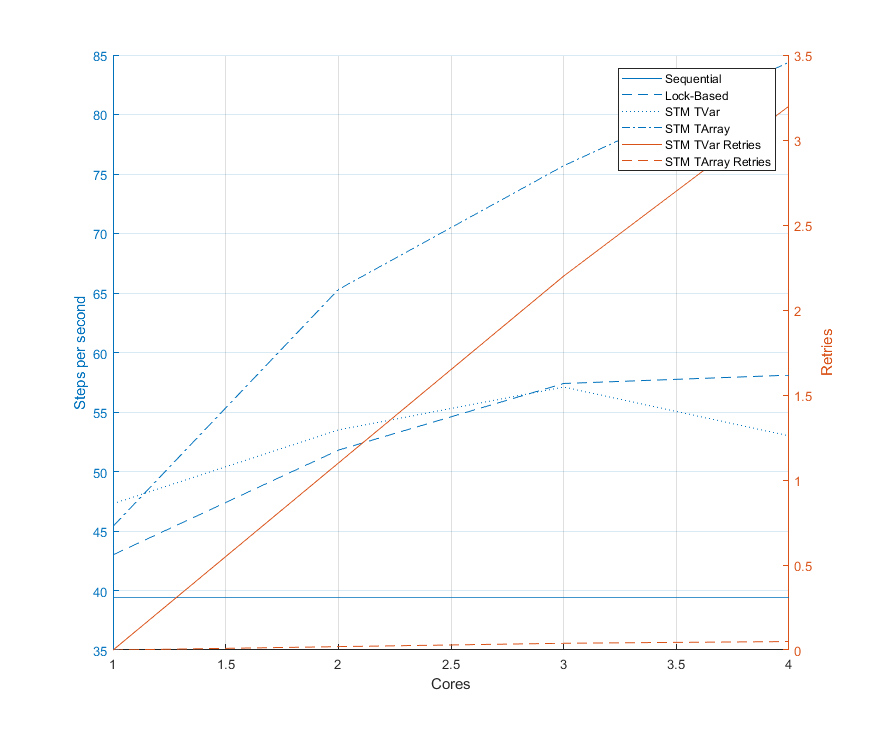
\includegraphics[width=0.7\textwidth, angle=0]{./fig/concurrentabs/sugarscape/varying_cores.png}
	\caption{Steps per second and retries on 50x50 grid and 500 initial agents on varying cores.}
	\label{fig:varying_cores}
\end{figure}

As expected, the \textit{Sequential} implementation is the slowest, followed by the \textit{Lock-Based} and \textit{TVar} approach whereas \textit{TArray} is the best performing one.

We clearly see that using a \textit{TVar} to share the environment is a very inefficient choice in this model: \textit{every} write to a cell leads to a retry independent whether the reading agent reads that changed cell or not, because the data-structure can not distinguish between individual cells. By using a \textit{TArray} we can avoid the situation where a write to a cell in a far distant location of the environment will lead to a retry of an agent which never even touched that cell. Also the \textit{TArray} seems to scale up by 10 steps per second for every core added. It will be interesting to see how far this could go with the Amazon experiment, as we seem not to hit a limit with 4 cores yet.

The inefficiency of \textit{TVar} is also reflected in the nearly similar performance of the \textit{Lock-Based} implementation which even outperforms it on 4 cores. This is due to very similar approaches because both operate on the whole environment instead of only the cells as \textit{TArray} does. This seems to be a bottleneck in \textit{TVar} reaching the best performance on 3 cores, which then drops on 4 cores due to an increasing retries ratio. The \textit{Lock-Based} approach seems to reduce its returns on increased number of cores hitting a limit at 4 cores as well.

\subsection{Scaling up Agents}
So far we kept the initial number of agents at 500, which due to the model specification, quickly drops and stabilises around 200 due to the carrying capacity of the environment as described in the book \cite{epstein_growing_1996} section \textit{Carrying Capacity} (p. 30).

We now want to measure the performance of our approaches under increased number of agents. For this we slightly change the implementation: always when an agent dies it spawns a new one which is inspired by the ageing and birthing feature of Chapter III in the book \cite{epstein_growing_1996}. This ensures that we keep the number of agents roughly constant (still fluctuates but doesn't drop to low levels) over the whole duration. This ensures a constant load of concurrent agents interacting with each other and demonstrates also the ability to terminate and create concurrent agents (threads) dynamically during the simulation.

Except for the \textit{Sequential} approach we ran all experiments with 4 cores (TVar with 3 as well). We looked into the performance of 500, 1,000, 1,500, 2,000 and 2,500 (maximum possible capacity of the 50x50 environment). The results are reported in Table \ref{tab:state_results_agentsscale_time} and plotted in Figure \ref{fig:state_results_agentsscale_time}.

\begin{table}
	\centering
  	\begin{tabular}{ c || c | c | c | c | c }
        Agents  & Sequential & Lock-Based & TVar (3 cores) & TVar (4 cores) & TArray  \\ \hline \hline 
    	    500     & 14.4       & 20.2		  &	20.1           & 18.5       	& \textbf{71.9}    \\ \hline
   		1,000   & 6.8        & 10.8 	      & 10.4           & 9.5         & \textbf{54.8}    \\ \hline
   		1,500   & 4.7        & 8.1 		  & 7.9            & 7.3			& \textbf{44.1}    \\ \hline
   		2,000   & 4.4        & 7.6 		  & 7.4            & 6.7    		& \textbf{37.0}    \\ \hline 
   		2,500   & 5.3        & 5.4 		  & 9.2            & 8.9			& \textbf{33.3}    \\ \hline \hline
   	\end{tabular}
  	
  	\caption{Steps per second on 50x50 grid with varying number of agents with 4 (and 3) cores except Sequential (1 core).}
	\label{tab:state_results_agentsscale_time}
\end{table}

\begin{figure}
	\centering
	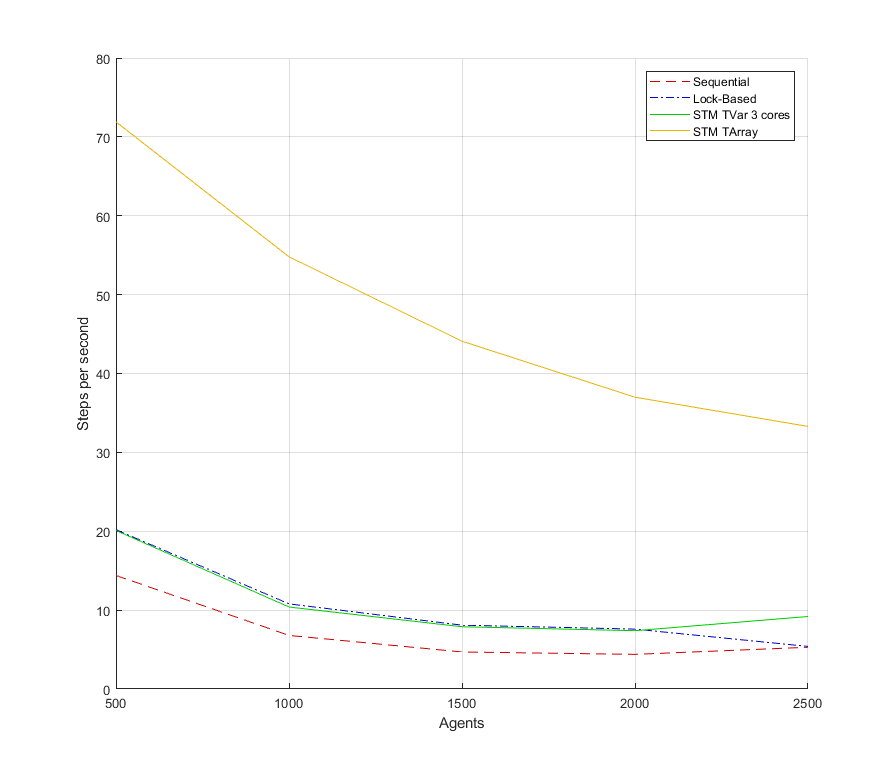
\includegraphics[width=1.0\textwidth, angle=0]{./fig/concurrentabs/sugarscape/varying_agents.png}
	\caption{Steps per second on 50x50 grid and varying number of agents with 4 (and 3) cores except Sequential (1 core).}
	\label{fig:state_results_agentsscale_time}
\end{figure}

As expected, the \textit{TArray} implementation outperforms all others substantially. Also as expected, the \textit{TVar} implementation on 3 cores is faster than on 4 cores as well when scaling up to more agents. The \textit{Lock-Based} approach performs about the same as the \textit{TVar} on 3 cores because of the very similar approaches: both access the \textit{whole} environment. Still the \textit{TVar} approach uses one core less to arrive at the same performance, thus strictly speaking outperforming the \textit{Lock-Based} implementation.

What seems to be very surprising is that in the \textit{Sequential} and \textit{TVar} cases the performance with 2,500 agents is \textit{better} than the one with 2,000 agents. The reason for this is that in the case of 2,500 agents, an agent can't move anywhere because all cells are already occupied. In this case the agent won't rank the cells in order of their pay-off (max sugar) to move to but just stays where it is. We hypothesize that due to Haskells laziness the agents actually never look at the content of the cells in this case but only the number which means that the cells themselves are never evaluated which further increases performance. This leads to the better performance in case of \textit{Sequential} and \textit{TVar} because both exploit laziness.
In the case of the \textit{Lock-Based} approach we still arrive at a lower performance because the limiting factor are the unconditional locks. In the case of the \textit{TArray} approach we also arrive at a lower performance because it seems that STM perform reads on the neighbouring cells which are not subject to lazy evaluation. In Haskell it is notoriously difficult to reason about efficiency (see Chapter \ref{ch:drawbacks} for a short discussion on drawbacks) and this behaviour of improved performance due to Haskells lazyness is no exception. We leave an in-depth investigation for further research as it is beyond the focus of this chapter.

We also measured the average retries both for \textit{TVar} and \textit{TArray} under 2,500 agents where the \textit{TArray} approach shows best scaling performance with 0.01 retries whereas \textit{TVar} averages at 3.28 retries. Again this can be attributed to the better transactional data-structure which reduces retry-ratio substantially to near-zero levels.

\subsection{Going Large-Scale}
To test how far we can scale up the number of cores in both the \textit{Lock-Based} and \textit{TArray} cases, we ran the two experiments (carrying capacity and rebirthing) on Amazon EC2 instances with increasing number of cores starting with 16 and 32 to see if we run into decreasing returns. The results are reported in Table \ref{tab:sug_varying_cores_amazon}.

\begin{table}
	\centering
%  	\begin{tabular}{ c || c | c | c }
%                   & Cores & Carrying Capacity & Rebirthing  \\ \hline \hline 
%    	Lock-Based & 16    & 53.9              & 4.4         \\ \hline
%    	Lock-Based & 32    & 44.2              & 3.6         \\ \hline \hline 
%   		
%   		STM TArray & 16    & \textbf{116.8} (0.23)      & \textbf{39.5} (0.08) \\ \hline
%   		STM TArray & 32    & 109.8 (0.41)      & 31.3 (0.18) \\ \hline \hline 
%   	\end{tabular}
  	
	\begin{tabular}{cc|c|c}
		\multicolumn{1}{ c||  }{\multirow{2}{*}{} } &
		\multicolumn{1}{ |c| }{Cores} & Carrying Capacity    & Rebirthing       \\ \hline \hline 
		
		\multicolumn{1}{ c||  }{\multirow{2}{*}{Lock-Based} } &
		\multicolumn{1}{ |c| }{16} & 53.9              & 4.4       \\ \cline{2-4}
		\multicolumn{1}{ c||  }{}                       &
		\multicolumn{1}{ |c| }{32} & 44.2              & 3.6      \\ \hline \hline 
		
		\multicolumn{1}{ c||  }{\multirow{2}{*}{STM TArray} } &
		\multicolumn{1}{ |c| }{16} & \textbf{116.8} (0.23)      & \textbf{39.5} (0.08)       \\ \cline{2-4}
		\multicolumn{1}{ c||  }{}                       &
		\multicolumn{1}{ |c| }{32} & \textbf{109.8} (0.41)      & \textbf{31.3} (0.18)      \\ \hline \hline 
	\end{tabular}  	
  	
  	\caption{Steps per second on varying cores on Amazon S2 Services.}
	\label{tab:sug_varying_cores_amazon}
\end{table}

As expected, the \textit{Lock-Based} approach doesn't scale up to many cores because each additional core brings more contention to the lock, resulting in even more decreased performance. This is particularly obvious in the rebirthing experiment because of the much larger number of concurrent agents. The \textit{TArray} approach returns better performance on 16 cores but fails to scale further up to 32 where the performance drops below the one with 16 cores. We indicated the retry-ratio in brackets and see that they roughly double from 16 to 32, which is the reason why performance drops as at this point. 

%the INCREASE in time can only happen due to more retries
%Carrying Capacity 16 core ~ 0.23 retry-ratio
%Carrying Capacity 32 core ~ 0.41 retry-ratio
%
%Rebirthing 16 core ~ 0.08 retry-ratio
%Rebirthing 32 core ~ 0.18 retry-ratio

\subsection{Comparison with other approaches}
The paper \cite{lysenko_framework_2008} reports a performance of 17 steps in RePast, 18 steps in MASON (both non-parallel) and 2,000 steps per second on a GPU on a 128x128 grid. Although our \textit{Sequential} implementation, which runs non-parallel as well, outperforms the RePast and MASON implementations of \cite{lysenko_framework_2008}, one must be very well aware that these results were generated in 2008, on current hardware of that time.

%When we run the SugarScape example of RePast with the same model parameters as ours on the same machine (see Table \ref{tab:machine_specs}) we arrive at roughly 450 steps per second - a factor of about 3.8 faster than even our STM \textit{TArray} implementation on 16 cores. This might seem quite shocking, even more so because RePast also performs visual output, rendering the SugarScape in every step. When scaling up the agents to 2,500 the RePast version arrives around roughly 95 steps per second which is still faster by a factor of 3 than our 4 core \textit{TArray} implementation. We attribute this substantial performance difference to the inherent performance difference of functional programming to imperative approaches as already outlined in the previous section. 

The very high performance on the GPU does not concern us here as it follows a very different approach than ours. We focus on speeding up implementations on the CPU as directly as possible without locking overhead. When following a GPU approach one needs to map the model to the GPU which is a delicate and non-trivial matter. With our approach we show that speed up with concurrency is very possible without the low-level locking details or the need to map to GPU. Also some features as bilateral trading between agents, where a pair of agents needs to come to a conclusion over multiple synchronous steps, is difficult to implement on a GPU whereas this is easily possible using STM.

Note that we kept the grid-size constant because we implemented the environment as a single agent which works sequentially on the cells to regrow the sugar. Obviously this doesn't really scale up on parallel hardware and experiments which we haven't included here due to lack of space, show that the performance goes down dramatically when we increase the environment to 128x128 with same number of agents which is the result of Amdahl's law where the environment becomes the limiting factor of the simulation. Depending on the underlying data-structure used for the environment we have two options to solve this problem. In the case of the \textit{Sequential} and \textit{TVar} implementation we build on an indexed array, which we can be updated in parallel using the existing data-parallel support in Haskell. In the case of the \textit{TArray} approach we have no option but to run the update of every cell within its own thread. We leave both for further research as it is out of scope of this paper.

\subsection{Discussion}
This case study showed clearly that besides being substantially faster than the \textit{Sequential} implementation, \textit{STM} is also able to perform considerably better than a \textit{Lock-Based} approach even in the case of a model with much higher complexity in agent behaviour and dramatically increased number of writes to the environment.
Further, this case study demonstrated that the selection of the right transactional data-structure is of fundamental importance when using \textit{STM}. Selecting the right transactional data-structure is very model-specific and can lead to dramatically different performance results.
In this case the \textit{TArray} performed best due to many writes but in the SIR case-study a \textit{TVar} showed good enough results due to the very low number of writes. When not carefully selecting the right transactional data-structure which supports fine-grained concurrency, a lock-based implementation might perform as well or even outperform the STM approach as can be seen when using the \textit{TVar}.
Although the \textit{TArray} is the better transactional data-structure overall, it might come with an overhead, performing worse on low number of cores than a \textit{TVar} approach but has the benefit of quickly scaling up to multiple cores. Depending on the transactional data-structure, scaling up to multiple cores hits a limit at some point. In the case of the \textit{TVar} the best performance is reached with 3 cores. With the \textit{TArray} we reached this limit around 16 cores.

Note that the comparison between the \textit{Lock-Based} approach and the \textit{STM TArray} implementation is a bit unfair due to a very different locking structure. A more suitable comparison would have been to use an indexed Array with a tuple of (MVar, IORef) in each cell to support fine-grained locking on cell-level. This would be a more just comparison to the \textit{STM Array} where fine-grained transactions happen on the cell-level. We hypothesize that \textit{STM} will still outperform the \textit{IO} approach but to a lesser degree - we leave the proof of this for further research.

%Unfortunately, for this model the performance is nowhere comparable to imperative approaches, which we attribute to the inherent performance difference of functional programming to imperative approaches. With the use of advanced language features we might arrive at much improved performance but we leave this for further research as we focus primarily on the comparison between lock-based and STM approaches.

%we can implement everything except synchronous direct agent-interactions atm: if agent-interaction is one-way e.g. paying back a loan then this is no problem. thus the following parts of the Sugarscape are not possible with our current STM approach: mating, trading and lending  because all 3 require direct agent-to-agent interaction over multiple steps. We leave the problem of developing such an algorithm / implementation for further research.

\section{Discussion}
Although there are similarities to the work of \cite{botta_time_2010} (the use of messages and the problem of when to advance time in models with arbitrary number synchronised agent-interactions), we approach our agents differently. First in our approach an agent is only a single MSF and thus can not be directly queried for its internal state / its id or outgoing messages, instead of taking a list of messages, our agents take a single event/message and can produce an arbitrary number of outgoing messages together with an observable state - note that this would allow to query the agent for its id and its state as well by simply sending a corresponding message to the agents MSF and requiring the agent to implement message handling for it. Also the state of our agents is \textit{completely} localised and there is no means of accessing the state from outside the agent, they are thus "fully encapsulated agents" \cite{botta_time_2010}. Note that the authors of \cite{botta_time_2010} define their agents with a polymorphic agent-state type \textit{s}, which implies that without knowledge of the specific type of \textit{s} there would be no way of accessing the state, rendering it in fact also fully encapsulated. The problem of advancing time in our approach is solved not exactly the same but conceptually it is the same: after sending a tick message to each agent (in random order), we process all agents until they are idle: there are no more enqueued messages / events in the queue.

our eventdriven approach makes heavy use of 2 state monads, thus one might ask what the benefits are, after all we seem to fall back into stateful, imperative style programming. we agree that our approach is just one way of implementing abs in fp but we think we have come a long way thus making our approach quite valuable even if there might be other approaches like shallow EDSLs. on the other hand even our stateful programming is highly restricted to only those 2 local datatypes which makes it much more manageable than unrestricted data mutation

quote carmack (\url{http://www.gamasutra.com/view/news/169296/Indepth_Functional_programming_in_C.php}): the main difficulty as a developer in software programming is to keep track of the states a program can be in and reason about them and their Validity

TODO: report LoC and compare it with other implementations we found on the internet